A análise de sentimento é uma técnica de processamento de linguagem natural que envolve a identificação e extração de informações subjetivas a partir de dados textuais. Esse processo pode ser usado para identificar a polaridade, ou tom emocional, de um determinado texto, o que pode ser útil em várias aplicações, como pesquisa de mercado e análise de mídias sociais \cite{2008_Pang}. Pesquisas anteriores demonstraram a utilidade da análise de sentimento em diversos domínios, incluindo política, negócios e saúde \cite{2016_Chen_IP}.

Técnicas de aprendizado de máquina podem ser usadas para automatizar o processo de análise de sentimento. Essas técnicas envolvem o treinamento de um modelo de aprendizado de máquina em um conjunto de dados rotulados, onde os rótulos indicam a polaridade dos dados textuais. Uma vez treinado, o modelo pode ser usado para prever a polaridade de novos dados textuais que não foram vistos anteriormente. Algoritmos de aprendizado de máquina comumente usados para análise de sentimento incluem regressão logística, máquinas de vetor de suporte e redes neurais \cite{2013_Haddi}.

Neste capítulo, abordamos a análise de sentimento como uma ferramenta poderosa no contexto do processamento de linguagem natural, focando especialmente nas postagens do Colab. Exploramos como técnicas de aprendizado de máquina, particularmente com o uso do Natural Language Toolkit (NLTK), podem ser empregadas para automatizar e aprimorar a análise de sentimentos. Além disso, discutimos a relevância de identificar diferentes "personas" de usuários, como os 'Helpers' e 'Complainers', e como essa distinção pode influenciar a dinâmica e a polarização dentro de uma plataforma de mídia social. Finalmente, abordamos a relação entre análise de sentimento, polarização e a formação de câmaras de eco, destacando a importância de entender e mitigar esses fenômenos em ambientes digitais.

\section{Processamento de linguagem natural e Análise de sentimento}

A análise de sentimento é uma técnica de processamento de linguagem natural amplamente utilizada para identificar e extrair informações subjetivas de dados textuais. Essa abordagem envolve a identificação da polaridade ou tom emocional presente em um determinado texto \cite{2008_Pang}, o que pode ser aplicado em diversas áreas, como pesquisa de mercado e análise de mídias sociais \cite{2015_Nguyen}.

Técnicas de aprendizado de máquina, como o uso do Natural Language Toolkit (NLTK), são frequentemente empregadas para automatizar o processo de análise de sentimento. O NLTK é uma biblioteca em Python que fornece uma ampla gama de ferramentas e recursos para tarefas de processamento de linguagem natural, incluindo a análise de sentimentos \cite{2009_Bird_BOOK}. Ele oferece uma variedade de recursos, como classificadores pré-treinados, dicionários léxicos, algoritmos de tokenização e técnicas de stemming.

Para realizar a análise de sentimento, aliamos o NLTK a dicionários léxicos, que são conjuntos de palavras pré-definidas associadas a uma polaridade de sentimento (positiva, negativa ou neutra). Esses dicionários podem ser usados para atribuir uma polaridade a palavras individuais em um texto e calcular a polaridade geral do texto com base nessas palavras \cite{2012_Souza_IP}. O NLTK oferece uma variedade de dicionários léxicos, como o VADER (Valence Aware Dictionary and sEntiment Reasoner), que é um dicionário léxico e uma ferramenta de análise de sentimento projetada especificamente para textos de mídia social \cite{2014_Hutto}. O VADER é um dos dicionários léxicos mais utilizados no contexto de análise de sentimento, pois foi projetado para lidar com as particularidades da linguagem utilizada em mídias sociais, como o uso de gírias, abreviações e emojis \cite{2014_Hutto}. No entanto, uma limitação significativa do VADER é sua incapacidade de processar e classificar eficazmente textos em português, dada sua orientação primária para o idioma inglês. Esta lacuna linguística pode resultar em análises imprecisas ou distorcidas quando aplicadas a conjuntos de dados predominantemente em português. Diante dessa problemática, optou-se pela incorporação do LeIA (Léxico para Inferência de Afinidade) como uma métrica complementar em nossa análise. O LeIA \cite{2018_Almeida_PAGE}, desenvolvido especificamente para o português, oferece uma dimensão adicional e mais adaptada à classificação das postagens do Colab, permitindo uma análise de sentimento mais robusta e contextualizada para o cenário brasileiro.

A análise de sentimento com o uso do NLTK geralmente segue um processo que envolve o pré-processamento dos textos, a tokenização (divisão em palavras ou frases), a atribuição de polaridade a cada palavra com base no dicionário léxico e o cálculo de uma pontuação geral de sentimento para o texto \cite{2013_Haddi}. Essa pontuação pode ser usada para classificar o texto como positivo, negativo ou neutro. Além disso, o NLTK oferece recursos adicionais para aprimorar a análise de sentimento, como a remoção de stop words (palavras comuns que geralmente não carregam um significado emocional) e a lematização (redução de palavras a sua forma básica, por exemplo, reduzir 'correndo' a 'correr'). Ao combinar as técnicas oferecidas pelo NLTK com algoritmos de aprendizado de máquina, como regressão logística, máquinas de vetor de suporte e redes neurais, é possível obter modelos de análise de sentimento mais sofisticados e precisos \cite{2014_Kim}.

No contexto específico do Colab, a análise de sentimento pode desempenhar um papel fundamental na detecção e mitigação da formação de câmaras de eco. Pesquisas anteriores têm demonstrado que a análise de sentimento pode ser utilizada para identificar as crenças e inclinações políticas dos usuários com base em sua linguagem e sentimentos expressos nas postagens de mídias sociais. Algoritmos de aprendizado de máquina, como Naive Bayes, Random Forest e Support Vector Machines (SVM), têm sido amplamente aplicados na análise de sentimento nesse contexto como por exemplo demonstrado em \citeonline{2014_Hutto}.

Para identificar câmaras de eco, a análise de sentimento pode ser usada como uma métrica para medir a homofilia em uma rede social. A homofilia se refere à tendência dos indivíduos de se associarem com outros que são semelhantes a eles em termos de características, opiniões e sentimentos. Ao analisar o sentimento expresso nas postagens dos usuários, podemos determinar se um grupo de usuários está polarizado, ou seja, se a maioria de suas postagens apresenta um sentimento ou inclinação política semelhante.

Além de identificar a polarização, a análise de sentimento também pode revelar os tópicos específicos que estão impulsionando a polarização dentro dessas câmaras de eco. Ao examinar o conteúdo das postagens e identificar os principais temas discutidos, é possível compreender melhor os fatores que contribuem para a formação e manutenção dessas câmaras de eco.

No contexto do Colab, este estudo propõe a introdução de duas métricas adicionais no modelo de dados dos usuários: score e persona. O score refere-se à classificação das postagens como positivas ou negativas, com base em dicionários léxicos. Essa abordagem tem sido aplicada em diversos domínios de negócios e sociais, uma vez que as opiniões desempenham um papel central em nossas atividades diárias e influenciam nossos comportamentos \cite{2012_Souza_IP}.

\subsection*{Análise de Sentimento, homofilia e polarização}

No contexto da polarização em redes sociais, a Análise de Sentimento é uma ferramenta poderosa para detectar e mitigar a formação de câmaras de eco. Pesquisas anteriores mostraram que a análise de sentimento pode ser usada para identificar as crenças e inclinações políticas dos usuários com base em sua linguagem e sentimento expressos em postagens de mídias sociais. Algoritmos de aprendizado de máquina, como Naive Bayes, Random Forest e Support Vector Machines (SVM), têm sido amplamente utilizados para análise de sentimento \cite{2014_Hutto}.

Para identificar câmaras de eco, a análise de sentimento pode ser usada como uma métrica para medir a homofilia em uma rede social. A homofilia refere-se à tendência dos indivíduos de se associarem com outros que são semelhantes a eles em termos de características, opiniões e sentimentos. Ao analisar o sentimento expresso nas postagens de usuários, podemos determinar se um grupo de usuários está polarizado, ou seja, se a maioria de suas postagens apresenta um sentimento ou inclinação política semelhante.

A análise de sentimento permite medir o grau de polarização dentro desse grupo, fornecendo uma medida quantitativa do nível de homofilia na rede. Se os usuários dentro de um grupo apresentarem predominantemente sentimentos semelhantes, isso indica uma maior homofilia e uma maior probabilidade de formação de uma câmara de eco.

Além de identificar a polarização, a análise de sentimento também pode revelar os tópicos específicos que estão impulsionando a polarização dentro dessas câmaras de eco. Ao examinar o conteúdo das postagens e identificar os principais temas discutidos, é possível compreender melhor os fatores que contribuem para a formação e manutenção dessas câmaras de eco.

Com essa abordagem, a análise de sentimento não apenas fornece insights sobre a polarização em uma rede social, mas também ajuda a identificar os grupos de usuários que estão mais propensos a formar câmaras de eco e a perpetuar a polarização. Essas informações são valiosas para a compreensão dos padrões de interação e para o desenvolvimento de estratégias de mitigação da polarização e promoção do diálogo diversificado e inclusivo.

Por exemplo, em um estudo de \citeonline{2014_Colleoni}, a análise de sentimento foi usada para medir a polarização de usuários em discussões políticas no Twitter. Os autores descobriram que os usuários tendem a se agrupar em torno de indivíduos com opiniões semelhantes e que esse agrupamento leva à formação de câmaras de eco. Os autores sugeriram que a análise de sentimento poderia ser usada para identificar os usuários que estão impulsionando a polarização e direcioná-los com contra-argumentos ou pontos de vista alternativos.

\section{Análise exploratória de Sentimento}

Neste capítulo, nos aprofundamos na análise de sentimentos das postagens do Colab, introduzindo a métrica de "score". Esta métrica foi desenvolvida especificamente para este estudo, com o intuito de classificar as postagens como positivas ou negativas, proporcionando uma visão mais quantitativa dos sentimentos expressos pelos usuários. Além disso, apresentamos uma análise exploratória dos dados, com o objetivo de identificar os principais tópicos discutidos no Colab e as principais palavras associadas a cada tópico. Por fim, adicionamos uma camada de análise de redes no experimento, introduzindo a assortatividade como uma métrica para medir a homofilia na rede.

Para realizar essa análise, fundamentamos nosso estudo em conceitos e técnicas de processamento de linguagem natural (PLN) e análise de sentimentwos. O PLN é uma área da inteligência artificial que visa capacitar os computadores a entender, interpretar e gerar linguagem humana de forma natural. A análise de sentimentos, por sua vez, é uma subárea do PLN que se concentra em identificar e extrair informações sobre os sentimentos e opiniões expressos em textos.

Utilizamos a linguagem de programação Python como base para a implementação do experimento. Como runtime, novamente utilizamos o Google Colab, que nos permite executar o código em nuvem, sem a necessidade de instalar bibliotecas ou configurar o ambiente de desenvolvimento. O código-fonte do experimento está disponível no GitHub\footnote{https://github.com/guinetik/colab-network-ec}.

Com a aplicação dessas técnicas e o uso da linguagem Python, pudemos extrair insights valiosos sobre os sentimentos presentes nas postagens do Colab. Essas métricas servirão como base para as análises subsequentes e contribuirão para aprimorar a compreensão do ecossistema do Colab.

\subsection{Classificação de postagens por Score}

No capítulo anterior, realizamos uma análise exploratória da rede, identificando comunidades de usuários e suas interações. Neste contexto, a classificação de postagens por score torna-se uma ferramenta valiosa. Esta métrica categoriza as postagens como positivas, negativas ou neutras com base em seu conteúdo textual, utilizando uma abordagem de pontuação de sentimentos. Cada postagem recebe um score de sentimento que varia de -1 (negativo) a 1 (positivo), com scores próximos a 0 indicando neutralidade. Esta abordagem quantitativa não só nos permite capturar o sentimento geral expresso nas postagens, mas também entender como esses sentimentos se propagam e interagem dentro da rede. Assim, podemos obter insights valiosos sobre a percepção dos usuários em relação a diferentes tópicos e como essa percepção influencia a estrutura e a dinâmica da rede.

Para uma análise mais aprofundada, é crucial preparar adequadamente os dados para a classificação supervisionada de sentimentos. Utilizamos técnicas avançadas de Processamento de Linguagem Natural (PLN) para analisar postagens do Colab. O objetivo é classificar as postagens de forma eficaz, com base em seu conteúdo textual. Para isso, empregamos a biblioteca Spacy para tarefas de PLN e a biblioteca NLTK para tokenização e lematização. Além disso, as bibliotecas pandas e matplotlib são utilizadas para manipulação e visualização de dados, respectivamente. Esta preparação meticulosa dos dados é fundamental para treinar um algoritmo de classificação robusto e preciso. O \autoref{codigo:lex_train} é um exemplo de aplicação de técnicas de \sigla{PLN}{Processamento de Linguagem Natural} e Análise de Sentimentos para criar um conjunto de dados de treinamento para um algoritmo de classificação de sentimentos. Os próximos parágrafos exploram as heurísticas e técnicas utilizadas para esse modelo de classificação.

\begin{figure}[!htb]
	\caption{Demonstração do mapa sintático de uma frase utilizando o pacote Stanza para NLP, Deplacy para grafo de dependências e matplotlib para renderização.}
	\label{fig:lexicon_breakdown}
	\centering
	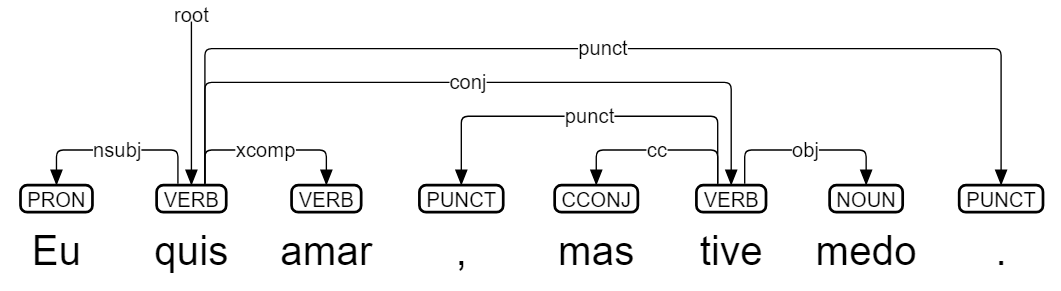
\includegraphics[scale=0.5]{images/lexicon_breakdown.png}
	\fautor
\end{figure}

A Análise de sentimentos emprega várias técnicas de \sigla{PLN}{Processamento de Linguagem Natural}, incluindo tokenização, lematização e remoção de palavras irrelevantes ou stop-words. A tokenização consiste em dividir o texto em palavras individuais ou "tokens". Já a lematização visa reduzir as palavras à sua forma base ou raiz, o que ajuda a consolidar diferentes formas da mesma palavra. Por sua vez, a remoção de palavras irrelevantes envolve a eliminação de termos comuns que geralmente não contribuem para o significado de uma frase, como "e", "o" e "em".Além dessas técnicas, a análise de sentimentos também se beneficia do uso de dicionários léxicos pré-existentes. Esses dicionários são valiosos recursos que contêm palavras associadas a valores de polaridade, indicando o sentimento geral de cada termo (positivo, negativo ou neutro).

No contexto da análise de sentimentos, existem vários dicionários léxicos relevantes disponíveis. Esse estudo comparou quatro repositórios bastante populares:

\begin{itemize}
	\item OpLexicon \cite{2011_Souza_IP}: É um dicionário léxico específico para o idioma português, com mais de 32.000 palavras, cada uma acompanhada de um valor de polaridade associado.
	\item SenticNet \cite{2016_Cambria_IP}: É dicionário léxico multilíngue que fornece valores de polaridade para palavras com base em sua semântica e psicologia.
	\item UniLex: Outro dicionário léxico multilíngue que oferece valores de polaridade para palavras com base em uma variedade de recursos linguísticos.
	\item WordNetAffectBR \cite{2008_Pasqualotti}: Esta é uma versão em português do WordNet-Affect, um dicionário léxico que atribui valores de polaridade às palavras com base em sua associação com diferentes emoções.
\end{itemize}

Ao utilizar esses dicionários léxicos, podemos comparar as palavras presentes no texto com as entradas nos dicionários para determinar a polaridade de cada uma. Isso nos possibilita obter uma compreensão mais abrangente dos sentimentos expressos no texto, contribuindo para uma análise de sentimentos mais precisa e eficaz. Esses dicionários são ferramentas valiosas no campo da análise de sentimentos, auxiliando na identificação e interpretação das emoções presentes nas palavras utilizadas. Além disso, com base nesses recursos, é possível automatizar e ampliar a análise de sentimentos em textos extensos, como avaliações de produtos, publicações em redes sociais e outros tipos de conteúdo textual.

Durante a comparação da polaridade da frase de teste com os dicionários léxicos, notou-se uma discrepância na normalização dos dicionários Unilex e WordNetAffectBR. Para este experimento, optamos por utilizar apenas o OpLexicon e o SenticNet, devido aos seus scores similares de polaridade e à presença de palavras exclusivas em cada um desses dicionários.

Além disso, realizamos um teste utilizando um \textit{subset} dos dados das postagens do Colab para adequação ao contexto. Durante esse teste, identificamos palavras relevantes que não estavam presentes nos dicionários léxicos originais. Adicionamos manualmente essas palavras ao conjunto de dicionários, atribuindo-lhes scores de -1 a 1 com base na polaridade observada nas postagens do Colab.

Em seguida, realizamos uma análise comparativa para avaliar a eficácia desses dicionários léxicos. Durante essa análise, calculamos a polaridade resultante para cada um dos dicionários, buscando identificar qual deles é mais eficaz na análise de sentimentos no contexto específico das postagens do Colab. Como resultado, obtivemos um amalgama dos dicionários OpLexicon e SenticNet, além do conjunto de palavras que foram adicionadas manualmente. Essas palavras foram normalizadas e incorporadas ao processo de análise.

O processo de análise de sentimento das postagens começa com o carregamento dos dados. Nessa análise, estamos interessados em postagens criadas por usuários das comunidades identificadas na análise do capítulo anterior, nas cidades de Niterói, Santo André e Mesquita. Em seguida, realizamos o pré-processamento do texto, que envolve a remoção de caracteres especiais, conversão para letras minúsculas, tokenização e aplicação de técnicas de stemização para reduzir as palavras às suas formas básicas \cite[]{2009_Bird_BOOK}.

Utilizamos a técnica de "bag-of-words" descrita em \citeonline{2013_Mikolov} com a biblioteca CountVectorizer para converter o texto em uma matriz numérica, onde cada coluna representa uma palavra e cada linha representa uma postagem. Com base nessa matriz, identificamos as palavras mais frequentes e as visualizamos em um gráfico de barras e na forma de uma nuvem de palavras.

\begin{figure}[!htb]
	\caption{Distribuição de palavras mais frequentes}
	\label{fig:wordcount}
	\centering
	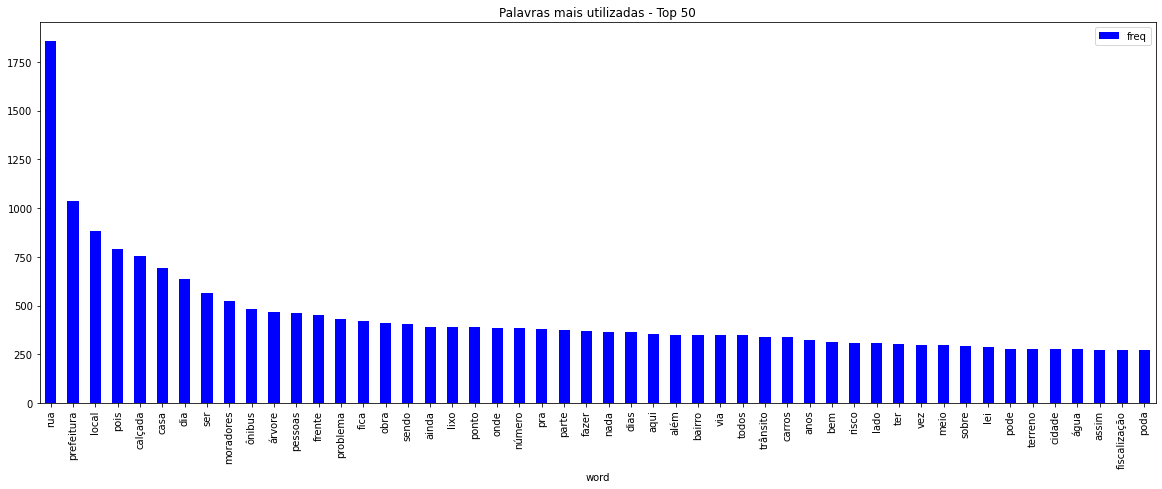
\includegraphics[scale=0.35]{images/wordcount.png}
	\fautor
\end{figure}

Realizamos uma análise exploratória dos dados para entender melhor as características das postagens. Isso incluiu a visualização da distribuição das palavras mais frequentes e a criação de nuvens de palavras para postagens positivas e negativas. Além disso, utilizamos a biblioteca Word2Vec para criar um modelo de palavras em vetores, que foi usado para visualizar as associações de palavras mais comuns.

\begin{figure}[!htb]
	\caption{Núvem de palavras mais utilizadas}
	\label{fig:wordcloud}
	\centering
	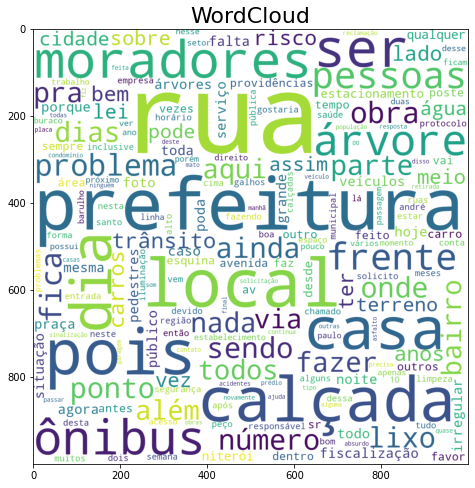
\includegraphics[scale=0.5]{images/wordcloud.png}
	\fautor
\end{figure}

\begin{figure}[htb]
	\centering
	\caption{Comparação de núvem de palavras mais usadas}\label{fig:lexicon_tagcloud}
	\begin{subfigure}[b]{0.317\textwidth}
		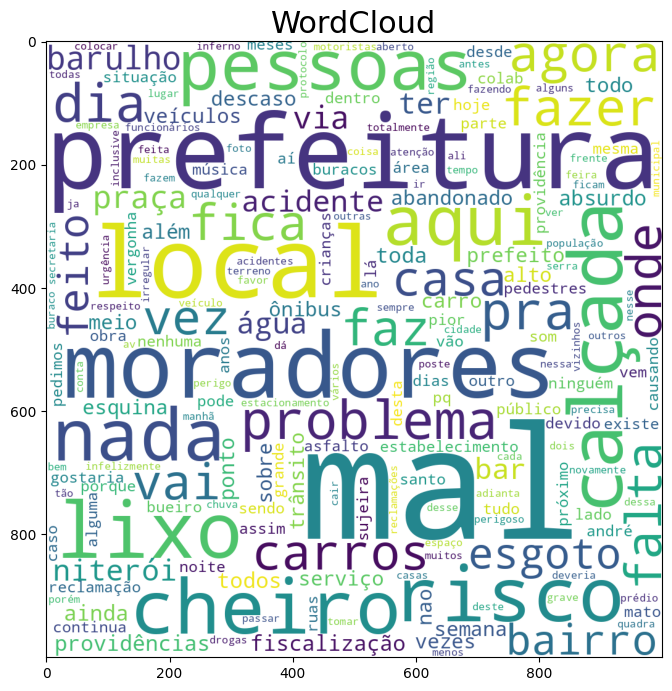
\includegraphics[width=\textwidth]{images/lexicon_worst_scores_tagcloud.png}
		\caption{Scores Negativos}
		\label{fig:tigre}
	\end{subfigure} ~ %add desired spacing between images, e. g. ~, \quad, \qquad, \hfill etc. %(or a blank line to force the subfigure onto a new line) 
	\begin{subfigure}[b]{0.317\textwidth}
		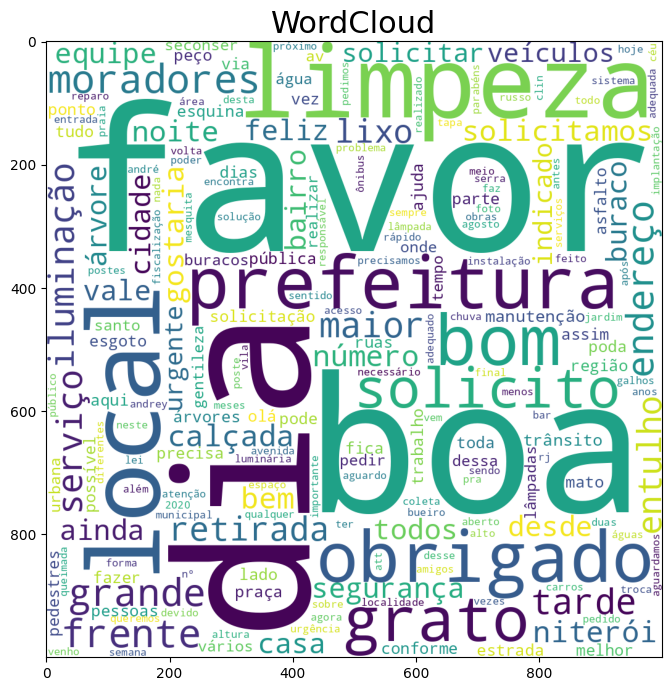
\includegraphics[width=\textwidth]{images/lexicon_best_scores_tagcloud.png}
		\caption{Scores Positivos} \label{fig:leao}
	\end{subfigure} ~ %add desired spacing between images, e. g. ~, \quad, \qquad, \hfill etc. %(or a blank line to force the subfigure onto a new line)
	\fautor
\end{figure}

Durante a análise exploratória, observamos uma tendência intrigante: muitos usuários optavam por se comunicar usando emojis. Em algumas instâncias, os emojis eram usados para complementar o texto, enquanto em outras, eles eram a principal forma de expressão. Isso levantou a questão sobre a polaridade sentimental desses emojis. Para abordar essa questão, recorremos ao dataset de sentimentos de emojis criado por \citeonline{2015_Novak}. Este conjunto de dados oferece uma classificação de sentimentos para emojis comuns, permitindo-nos incorporar essa dimensão em nossa análise.

Além dos emojis, notamos a presença de jargões específicos frequentemente usados pelos usuários do aplicativo. Estes jargões, muitas vezes, carregavam um significado ou conotação que não era imediatamente claro para quem não estava familiarizado com o contexto do aplicativo. Reconhecendo a importância desses jargões na análise de sentimentos, decidimos classificar manualmente a polaridade dos 100 jargões mais comuns encontrados no app. Isso também incluiu a identificação e classificação de nomes de partidos políticos, dada a sua relevância no discurso dos usuários.

Outro aspecto que chamou nossa atenção foi a presença de profanidades nas postagens. A linguagem ofensiva ou abusiva pode ter um impacto significativo na polaridade de uma postagem. Portanto, introduzimos uma etapa adicional em nossa análise para detectar essas profanidades. Ao identificá-las, classificamos essas palavras com uma polaridade negativa, garantindo que sua presença influenciasse adequadamente o score de sentimento da postagem em questão. Com essas etapas adicionais, buscamos uma análise de sentimentos mais robusta e contextualizada, levando em consideração as peculiaridades e nuances do discurso dos usuários no aplicativo.

Na busca por uma análise mais refinada e contextualizada dos sentimentos expressos nas postagens do Colab, decidimos incorporar uma métrica adicional ao nosso estudo: a análise de sentimentos realizada pelo pacote LeIA \cite{2018_Almeida_PAGE}. A inclusão dessa ferramenta visa aprimorar a nossa abordagem ao oferecer uma análise mais nuanceada dos sentimentos expressos nos textos, levando em consideração aspectos como a presença de emojis e a estrutura linguística das frases.

A ferramenta LeIA, desenvolvida especificamente para a língua portuguesa, apresenta uma abordagem que vai além da simples classificação de palavras individuais, oferecendo uma análise sintática e semântica mais profunda dos textos. Através da análise de sentimentos realizada pelo LeIA, obtemos uma pontuação composta (compound) que varia de -1 a +1, indicando o sentimento geral do texto, além de valores percentuais que representam a proporção de sentimentos positivos, negativos e neutros presentes no texto.

Para integrar essa métrica ao nosso estudo, adaptamos nossa função de análise de sentimentos para incluir a análise realizada pelo LeIA. Cada postagem do dataset foi analisada individualmente, gerando scores detalhados que incluem as métricas de positividade, negatividade, neutralidade e a pontuação composta. Esses scores foram então adicionados ao nosso dataset, prefixados com "leia" para indicar sua origem.

A decisão de integrar as métricas provenientes dos dicionários léxicos com as fornecidas pelo LeIA é motivada pela busca de uma análise mais holística e robusta. Enquanto nossos dicionários léxicos oferecem uma vasta base de palavras já classificadas, proporcionando uma análise ampla e generalizada, o LeIA traz uma perspectiva mais detalhada e contextual, capaz de interpretar nuances e particularidades da língua portuguesa, como a influência de emojis e a presença de negações no sentimento expresso. No entanto, é crucial reconhecer que tanto os dicionários léxicos quanto o LeIA podem introduzir seus próprios vieses na análise. Ao combinar essas métricas, aspiramos mitigar esses vieses individuais, buscando uma representação mais neutra e equilibrada dos sentimentos. A métrica composta, nesse contexto, não só permite uma categorização mais fluida dos sentimentos, evitando a rigidez das categorizações binárias, mas também proporciona uma visão mais matizada e imparcial dos dados.

Ao explorar a sinergia entre as métricas tradicionais e a análise realizada pelo LeIA, estamos em busca de respostas para uma questão central: como podemos, através da combinação de diferentes técnicas de análise de sentimentos, alcançar uma representação mais fiel e detalhada dos sentimentos expressos pelos usuários? Acreditamos que essa abordagem multidimensional pode revelar padrões e insights que seriam invisíveis através de uma única métrica. No entanto, é crucial enfatizar que a combinação de métricas apresenta desafios intrínsecos, sobretudo no que tange à calibração e à interpretação dos resultados. A integração das métricas não é uma simples concatenação de valores; ela demanda um processo meticuloso de normalização. Em nosso estudo, realizamos uma normalização dos scores para assegurar que as métricas provenientes de diferentes fontes estivessem em uma escala comum e comparável. Esse processo é fundamental para garantir que a combinação dos scores preserve a integridade e a precisão da análise, permitindo uma interpretação coesa e coerente dos sentimentos expressos nas postagens.

Para validar nossa abordagem, planejamos realizar uma série de testes e análises exploratórias, buscando entender como as métricas combinadas podem oferecer uma visão mais completa e rica dos sentimentos expressos nas postagens do Colab. Através dessa análise multidimensional, aspiramos a desvendar as complexidades do discurso dos usuários, oferecendo insights valiosos para a compreensão das dinâmicas sociais e emocionais presentes na plataforma.

Ao analisar a amostra fornecida, notamos que a combinação de métricas não apenas amplia a perspectiva sobre o sentimento, mas também ajuda a identificar nuances que poderiam ser perdidas se confiássemos em uma única métrica. Por exemplo, enquanto o score derivado dos dicionários léxicos pode capturar a polaridade geral de uma postagem, o leia\_compound do LeIA pode identificar sutilezas, como a influência de emojis ou a presença de negações, que podem alterar significativamente a interpretação do sentimento.

Além disso, observamos que a métrica composta compound\_score oferece uma visão mais equilibrada e matizada do sentimento. Em casos onde o score e o leia\_compound divergem, o compound\_score serve como uma espécie de "árbitro", proporcionando uma avaliação que leva em consideração ambas as perspectivas. Isso é particularmente útil em postagens onde o sentimento é ambíguo ou onde diferentes aspectos da postagem sugerem sentimentos contrastantes.

Outro insight interessante é a maneira como o compound\_score pode ajudar a identificar postagens que são particularmente polarizadas ou que geram sentimentos mistos. Postagens com compound\_scores próximos de zero, por exemplo, podem indicar postagens que contêm elementos tanto positivos quanto negativos, sugerindo que elas são mais complexas e merecem uma análise mais aprofundada.

Além disso, ao combinar métricas, também estamos abordando potenciais vieses inerentes a cada abordagem individual. Enquanto os dicionários léxicos podem ter suas próprias limitações e preconceitos, o LeIA, sendo uma ferramenta de aprendizado de máquina, pode ter seus próprios vieses com base nos dados com os quais foi treinado. Ao combinar essas métricas, esperamos criar uma métrica mais robusta e imparcial.

Em conclusão, ao adotar uma abordagem multidimensional para a análise de sentimentos, estamos não apenas buscando uma representação mais precisa do sentimento, mas também tentando entender as complexidades e nuances do discurso dos usuários. Esta abordagem combinada promete oferecer insights mais ricos e detalhados, permitindo uma compreensão mais profunda das emoções e opiniões expressas na plataforma Colab.

\subsubsection*{Análise de sentimento nas redes de Niterói, Santo André e Mesquita}

\begin{figure}[!htb]
	\caption{Distribuição dos scores de sentimento nas postagens da rede das 3 cidades selecionadas. Cada ponto representa um usuário e a cor indica o score médio de sentimento de suas postagens (verde para positivo, vermelho para negativo e laranja para neutro)}
	\label{fig:scores_scatterplot}
	\centering
	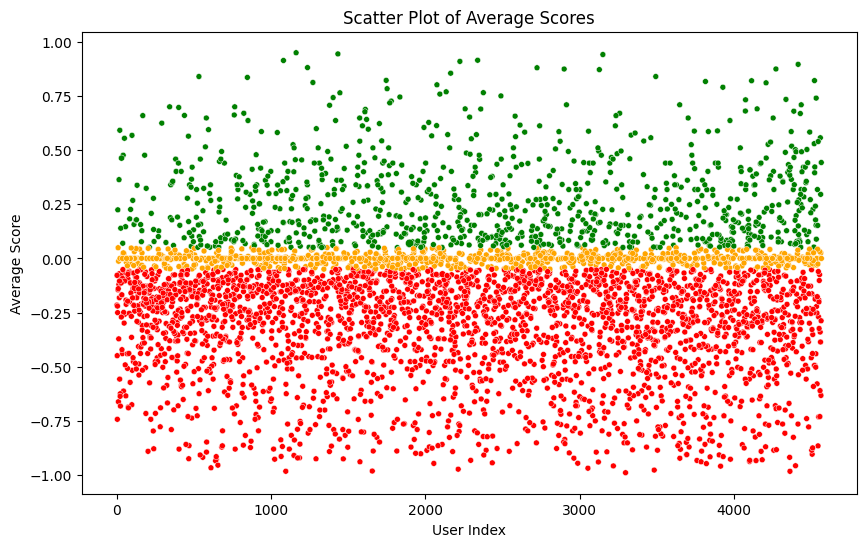
\includegraphics[scale=0.70]{images/scores_scatterplot.png}
	\fautor
\end{figure}

Após a seleção das postagens dos usuários das comunidades das cidades de Niterói, Santo André e Mesquita, conforme detalhado no capítulo anterior, foi possível identificar um total de 132.846 eventos de zeladoria criados por membros dessas comunidades. Esta vasta quantidade de dados nos ofereceu uma oportunidade única para aprofundar nossa análise de sentimentos e entender melhor as emoções e opiniões expressas pelos usuários.

Ao aplicar a análise de sentimentos nas postagens, foi essencial considerar a extensão dos textos. Uma postagem mais longa tem naturalmente mais palavras e, consequentemente, uma maior soma de polaridades. Para contornar essa característica e garantir uma análise justa, optamos por normalizar os scores com base no número de tokens ou palavras presentes na frase original. Esta abordagem permitiu que cada palavra contribuísse proporcionalmente para o score final da postagem, independentemente do seu tamanho.

Ao examinar os melhores scores, notamos algumas tendências interessantes. Primeiramente, as postagens com os scores mais elevados tendem a ter uma combinação de sentimentos neutros e positivos, conforme indicado pelas métricas do LeIA. Por exemplo, a postagem do evento 100876, originada de Niterói, apresenta uma combinação de 75,1\% de conteúdo neutro e 16,8\% de conteúdo positivo, resultando em um score composto de 0,671. Isso sugere que, mesmo quando os usuários estão apresentando informações factuais ou descritivas, há uma inclinação positiva em suas expressões.

Além disso, é notável que, mesmo com variações nos scores derivados dos dicionários léxicos, o LeIA consistentemente percebeu essas postagens como altamente positivas. Isso pode ser atribuído à capacidade do LeIA de capturar nuances e contextos específicos da língua portuguesa, como a influência de emojis e a presença de negações.

Outro ponto de destaque é a variedade de temas abordados nas postagens com os melhores scores. Enquanto algumas postagens, como a do evento 321209 de Santo André, focam em questões de zeladoria como o acúmulo de lixo, outras, como a do evento 328652, discutem colaborações entre organizações privadas e públicas. Isso reforça a ideia de que a plataforma Colab é um espaço diversificado, onde os usuários se sentem empoderados para discutir uma ampla gama de tópicos relacionados à melhoria de suas comunidades.

Em resumo, a análise dos melhores scores nos proporcionou uma visão mais clara das emoções e opiniões dos usuários nas comunidades selecionadas. Estes insights são fundamentais para entender as motivações dos usuários ao interagir na plataforma e podem ser usados para orientar futuras estratégias de engajamento e moderação.

\begin{figure}[!htb]
	\caption{Score médio de sentimento por número de usuários}
	\label{fig:average_score_by_number_of_users}
	\centering
	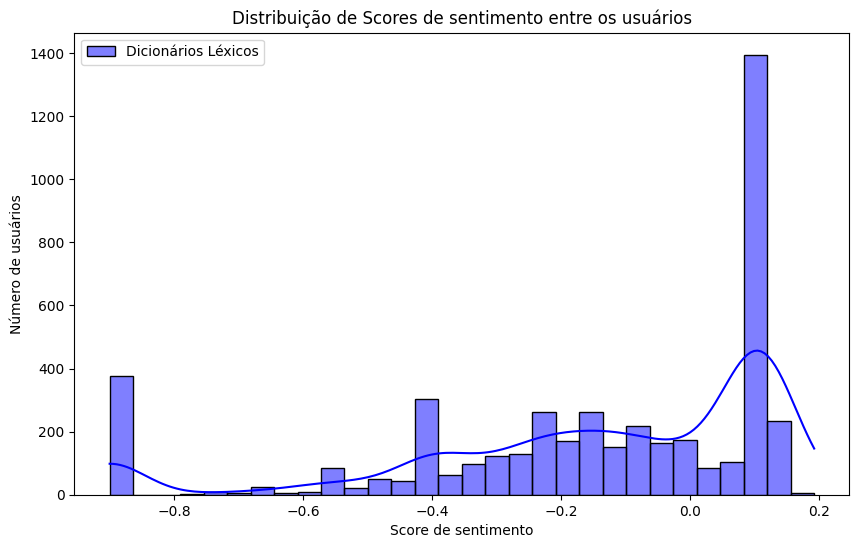
\includegraphics[scale=0.70]{images/average_score_by_number_of_users.png}
	\fautor
\end{figure}

Ao analisar os piores scores, é evidente que as postagens refletem um alto grau de insatisfação e frustração dos usuários em relação a questões específicas de zeladoria em suas comunidades. Estas postagens, oriundas das cidades de Niterói e Rio de Janeiro, destacam-se não apenas pelo conteúdo negativo, mas também pela intensidade das emoções expressas.

A postagem do evento 218258, por exemplo, menciona a repetição de reclamações feitas pelo usuário sem a devida solução, indicando um sentimento de desamparo e descontentamento com a resposta (ou falta dela) das autoridades competentes. O score derivado do dicionário léxico para esta postagem foi de -2.857, enquanto o LeIA identificou uma predominância de conteúdo neutro (73,5\%), mas com uma porcentagem significativa de conteúdo negativo (19,9\%). O score composto, que combina ambas as métricas, resultou em -0.957, refletindo a natureza altamente negativa da postagem.

Da mesma forma, a postagem do evento 156161 expressa indignação com a situação de uma rua específica, usando palavras em caixa alta para enfatizar o descontentamento. O uso de termos como "ABSURDO" e "CAOS" sugere uma forte emoção negativa. O LeIA capturou essa nuance, atribuindo um score negativo de -0.9930, enquanto o score do dicionário léxico foi de -0.167. A combinação de ambos resultou em um score composto de -0.956.

É interessante notar que, mesmo nas postagens com os piores scores, ainda há uma presença de conteúdo neutro e, em alguns casos, até mesmo positivo. Por exemplo, a postagem do evento 239454, apesar de expressar frustração com tentativas repetidas de comunicação, ainda contém uma saudação cordial ("Olá prezados"). Isso sugere que, mesmo em meio à insatisfação, os usuários ainda buscam manter um tom respeitoso e construtivo em suas comunicações.

Em resumo, as postagens com os piores scores ilustram claramente os desafios e frustrações enfrentados pelos usuários em suas comunidades. Estas postagens são valiosas, pois destacam áreas que requerem atenção imediata e melhorias por parte das autoridades locais. Além disso, a análise de sentimentos fornece uma ferramenta poderosa para identificar e compreender essas preocupações, permitindo uma resposta mais eficaz e empática por parte dos tomadores de decisão.

Após obter o score de sentimento de cada postagem, o próximo passo foi agregar as postagens de cada usuário. Ao calcular a média ponderada do score de sentimento pelo número de postagens, conseguimos criar um score geral que reflete o sentimento médio de todas as postagens de um usuário. Esta métrica agregada nos forneceu uma visão mais clara do panorama geral dos sentimentos expressos nas redes de Niterói, Santo André e Mesquita.

\begin{figure}[htbp]
	\centering
	\begin{subfigure}{0.45\textwidth}
		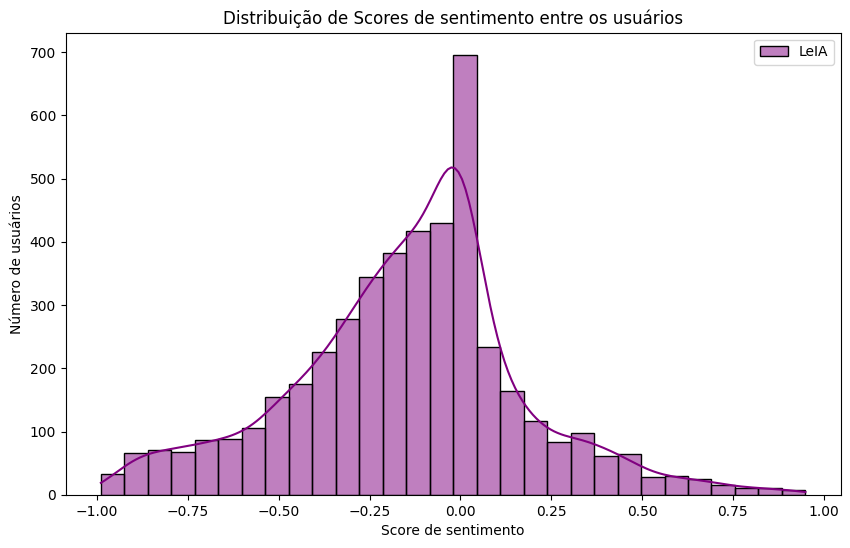
\includegraphics[width=\linewidth]{images/average_leia_by_number_of_users.png}
		\caption{Score Composto LeIA}
		\label{fig:average_leia_by_number_of_users}
	\end{subfigure}
	\hfill
	\begin{subfigure}{0.45\textwidth}
		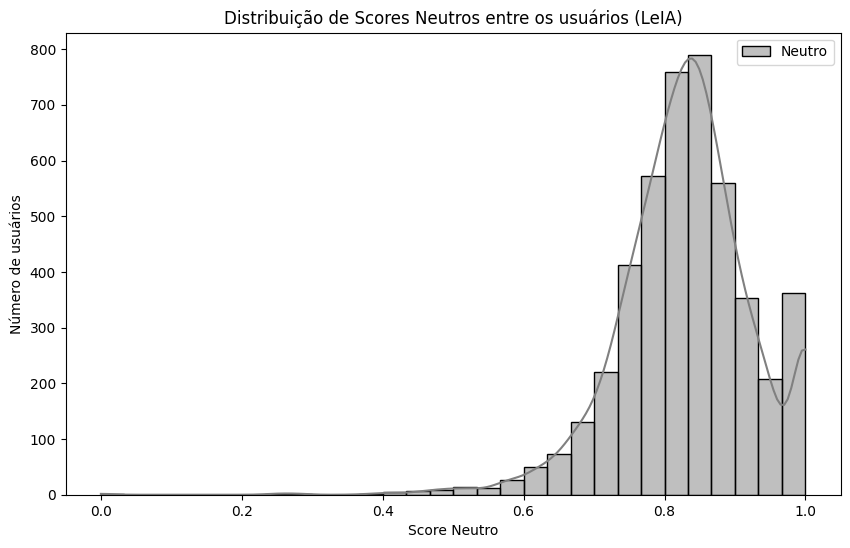
\includegraphics[width=\linewidth]{images/average_neutral_by_number_of_users.png}
		\caption{Neutros}
		\label{fig:average_neutral_by_number_of_users}
	\end{subfigure}
	\vskip\baselineskip
	\begin{subfigure}{0.45\textwidth}
		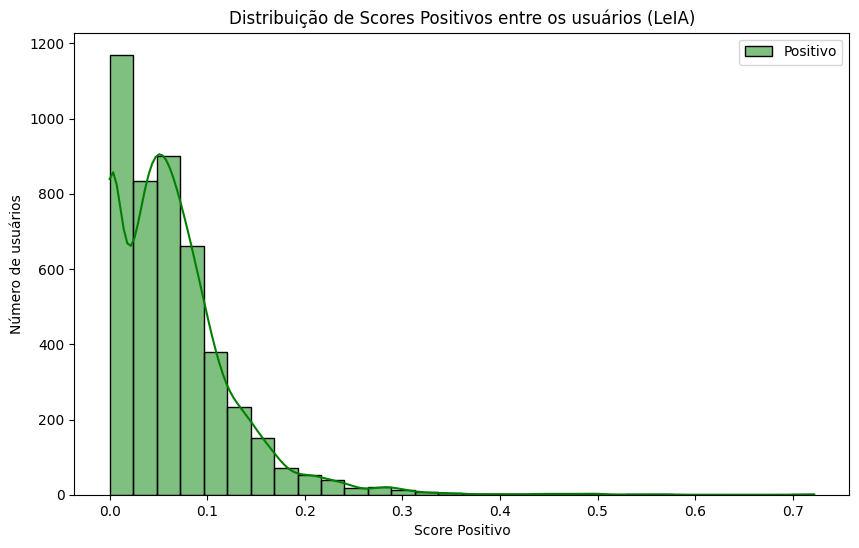
\includegraphics[width=\linewidth]{images/average_positive_by_number_of_users.png}
		\caption{Positivos}
		\label{fig:imagem3}
	\end{subfigure}
	\hfill
	\begin{subfigure}{0.45\textwidth}
		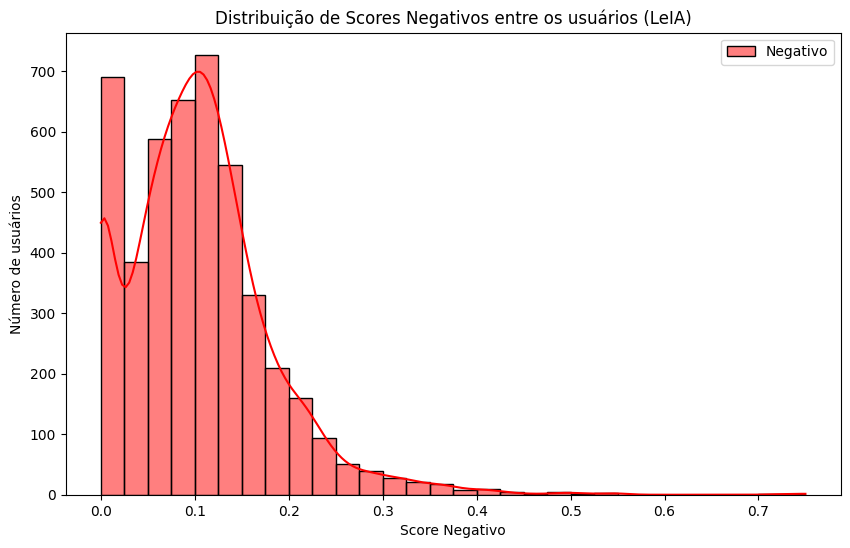
\includegraphics[width=\linewidth]{images/average_negative_by_number_of_users.png}
		\caption{Negativos}
		\label{fig:average_negative_by_number_of_users}
	\end{subfigure}
	\caption{Distribuição dos sentimentos médios em relação ao número de usuários. Os gráficos apresentam uma análise detalhada dos sentimentos, incluindo o score composto pelo LeIA, bem como as categorias neutras, positivas e negativas.}
	\label{fig:average_sentiment_by_number_of_users}
\end{figure}

Com os scores de sentimentos devidamente ajustados, partimos para uma análise mais detalhada dos dados. Uma observação inicial revelou que, ao contrário da premissa inicial de que a maioria das postagens tinha um tom negativo, a distribuição de sentimentos, quando consideramos cada postagem individualmente, mostra que 55.9\% das postagens são positivas, 24\% são negativas e 20.2\% são neutras. No entanto, quando agregamos todas as postagens de um único usuário, observamos que cerca de 67.3\% dos usuários têm postagens majoritariamente positivas, 17.7\% são majoritariamente negativas e 15\% são neutras.

Isso sugere que, embora possa haver uma percepção predominante de que os usuários expressam insatisfação ou preocupações em suas postagens, a realidade é mais matizada. A maioria dos usuários, de fato, tende a compartilhar feedbacks ou observações positivas sobre suas comunidades. Isso pode ser um reflexo de uma série de fatores: talvez os usuários estejam mais inclinados a compartilhar experiências positivas para promover a coesão comunitária, ou talvez as plataformas de mídia social, como o Colab, estejam se tornando espaços onde as pessoas desejam destacar o que está funcionando bem, em vez de apenas apontar problemas.

No entanto, os 24\% de postagens negativas não devem ser negligenciados. Mesmo que representem uma minoria em relação às postagens positivas, elas são cruciais para entender as áreas de preocupação e insatisfação dos usuários. Essas postagens podem ser extremamente valiosas para os tomadores de decisão, pois fornecem insights diretos sobre onde as intervenções podem ser mais necessárias.

As postagens neutras, que compõem 20.2\% do total, também são intrigantes. Elas podem representar uma variedade de conteúdos, desde solicitações de informação até comentários que não expressam uma opinião clara em uma direção ou outra. Essas postagens podem servir como um lembrete de que nem todo feedback pode ser facilmente categorizado como positivo ou negativo, e que a neutralidade em si pode oferecer insights sobre as áreas onde os sentimentos dos usuários são mistos ou incertos.

\begin{figure}[!htb]
	\caption{Scores de sentimento por quantidade de postagens}
	\label{fig:pie_sentiment_breakdown}
	\centering
	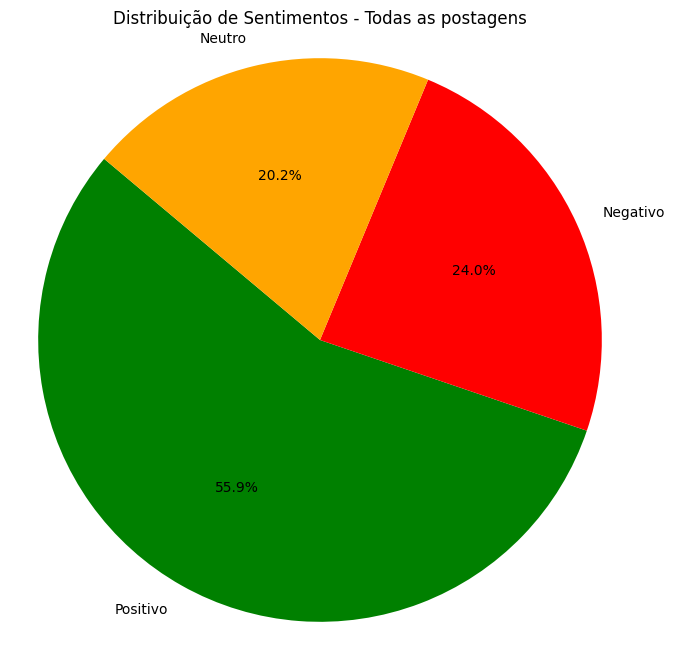
\includegraphics[scale=0.7]{images/pie_sentiment_breakdown.png}
	\fautor
\end{figure}

Ao analisar os eventos postados, observamos que "Entulho na calçada/via pública" é um dos tópicos mais frequentemente mencionados, com um total de 44.273 postagens. No entanto, é interessante notar que a maioria dessas postagens é classificada como neutra, com 35.391 postagens, seguida por 5.712 postagens positivas e 3.170 postagens negativas. Isso sugere que, embora haja uma alta incidência de relatos sobre entulho nas vias, muitos usuários não expressam uma opinião fortemente positiva ou negativa sobre o assunto.

Outro evento que se destaca é "Lâmpada apagada à noite", com um total de 8.701 postagens. Deste total, 3.212 postagens foram classificadas como neutras, 2.296 como positivas e 3.193 como negativas. Isso indica que há uma divisão nas opiniões dos usuários sobre a questão da iluminação pública à noite, com muitos reconhecendo os esforços para resolver o problema, mas também uma quantidade significativa de postagens expressando insatisfação.

Por outro lado, "Ponto de travessia irregular" teve um total de 46 postagens, das quais 31 foram classificadas como negativas, 6 como neutras e 6 como positivas. Isso sugere que há uma preocupação predominante com a segurança dos pontos de travessia, e que muitos usuários veem isso como uma área que precisa de melhorias.

Em resumo, os dados refletem as preocupações dos cidadãos em relação a diferentes aspectos da infraestrutura e serviços públicos. Enquanto alguns eventos são amplamente reportados e recebem uma mistura de feedback positivo, negativo e neutro, outros eventos, embora menos frequentemente mencionados, destacam-se por ter uma opinião predominantemente negativa ou positiva.

\begin{figure}[!htb]
	\caption{Distribuição dos 10 eventos mais comuns nas redes das 3 cidades.}
	\label{fig:pie_most_common_events}
	\centering
	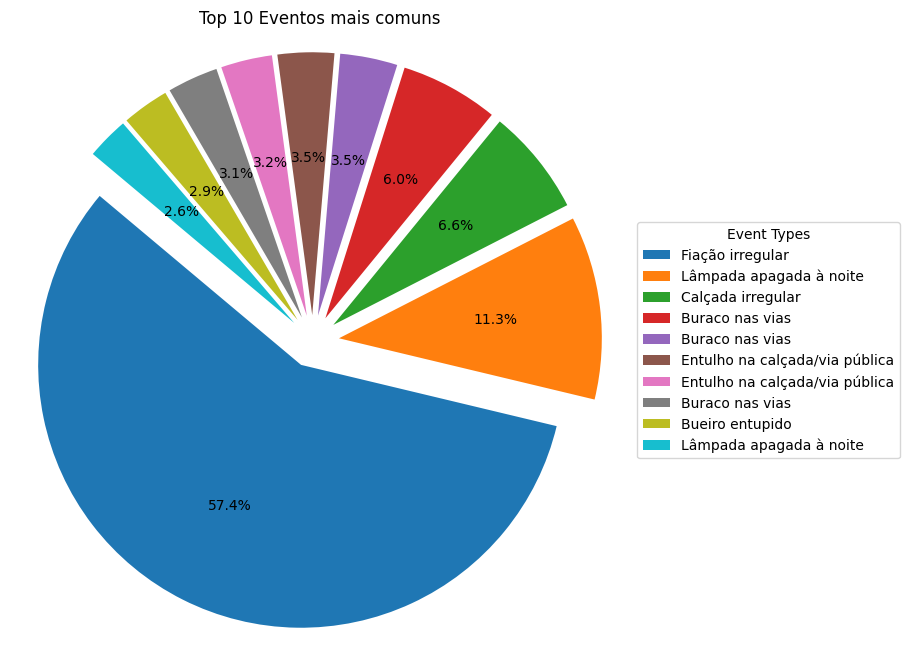
\includegraphics[scale=0.65]{images/pie_most_common_events.png}
	\fautor
\end{figure}

Ao expandir nossa análise para considerar a dimensão de gênero, observamos padrões distintos na distribuição de sentimentos entre diferentes grupos. Para as usuárias identificadas como femininas, notamos que a maioria das postagens (8.207) tem um sentimento negativo, seguido por 3.894 postagens positivas e 3.531 neutras. Isso sugere que, embora as mulheres estejam ativamente envolvidas na plataforma, elas tendem a expressar mais preocupações ou insatisfações em suas postagens do que sentimentos positivos ou neutros. Os usuários masculinos, por outro lado, apresentam um padrão diferente. Com 56.011 postagens neutras, 34.836 negativas e 22.513 positivas, vemos que a maioria das postagens masculinas é neutra. Isso pode indicar que os homens na plataforma tendem a ser mais informativos ou questionadores em suas postagens, sem expressar uma opinião clara em uma direção ou outra. Quanto aos usuários não binários, a amostra é extremamente pequena, com apenas uma postagem neutra registrada. Isso pode ser devido a uma representação limitada desse grupo na plataforma ou à relutância em se identificar devido a preocupações de privacidade. Os usuários que optaram por não informar seu gênero ou se identificaram como "outros" também têm uma presença na plataforma, embora em números menores em comparação com os gêneros masculino e feminino. Para os não informados, a distribuição é de 101 postagens negativas, 42 positivas e 37 neutras. Já para os que se identificam como "outros", temos 1.780 postagens negativas, 526 positivas e 1.356 neutras.

Essa análise por gênero destaca a importância de considerar as diversas perspectivas e experiências dos usuários ao avaliar o sentimento nas postagens. Cada grupo traz uma lente única para a plataforma, e entender essas nuances pode ajudar a criar estratégias de engajamento mais eficazes e a responder de forma mais adequada às preocupações e feedbacks dos usuários.

\begin{figure}[!htb]
	\caption{Distribuição dos scores de sentimento por gênero.}
	\label{fig:sentiment_by_gender}
	\centering
	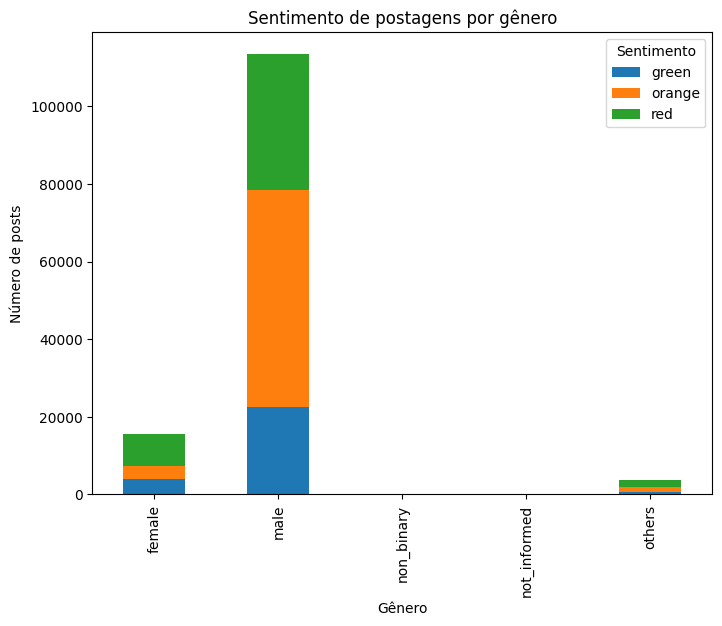
\includegraphics[scale=0.75]{images/sentiment_by_gender.png}
	\fautor
\end{figure}

Aprofundando ainda mais nossa análise, decidimos explorar a relação entre a análise de sentimentos e a estrutura da rede social do Colab. A ideia era entender como os sentimentos expressos nas postagens poderiam influenciar ou ser influenciados pelas conexões e interações entre os usuários. Neste contexto, a análise de redes sociais, combinada com a análise de sentimentos, pode oferecer insights valiosos sobre a formação e a dinâmica de câmaras de eco dentro da plataforma.

Um conceito fundamental na análise de redes é a assortatividade, que mede a tendência de nós em uma rede se conectarem a outros nós que são semelhantes em alguma característica específica. No nosso caso, estávamos interessados em entender se usuários com sentimentos semelhantes tendem a se conectar e interagir mais entre si.

\begin{table}[h]
	\centering
	\begin{tabular}{|l|c|}
		\hline
		\textbf{Atributo} & \textbf{Valor de Assortatividade} \\
		\hline
		Tipo de Evento    & 0.015                             \\
		\hline
		Idade             & 0.015                             \\
		\hline
		Gênero            & 0.025                             \\
		\hline
		Escolaridade      & 0.01987                           \\
		\hline
		Raça              & 0.025                             \\
		\hline
		Score Lexicon     & 0.01489                           \\
		\hline
		Score Composto    & 0.01489                           \\
		\hline
		Score Positivo    & 0.01487                           \\
		\hline
		Score Negativo    & 0.01489                           \\
		\hline
		Score Neutro      & 0.01489                           \\
		\hline
		Cidade            & 0.02506                           \\
		\hline
	\end{tabular}
	\caption{Assortatividade por Atributo}
\end{table}

Para entender a influência dos sentimentos nas conexões entre os usuários, começamos por calcular a assortatividade da rede em relação a várias características, incluindo o tipo de evento, idade, gênero, educação, raça, score médio de sentimento e cidade. A assortatividade nos fornece uma métrica quantitativa que indica se a rede exibe uma tendência de homofilia, ou seja, se nós semelhantes tendem a se conectar entre si.

Os resultados foram reveladores. Os resultados foram reveladores. A assortatividade para todas as características listadas variou entre 0.01487 e 0.02506, indicando uma tendência moderada de homofilia na rede. Em outras palavras, há uma leve tendência para usuários com características semelhantes se conectarem entre si.

O atributo 'gênero' e 'raça' apresentaram valores de assortatividade de 0.025, sugerindo que os usuários tendem a se conectar mais frequentemente com outros usuários do mesmo gênero ou raça. Da mesma forma, o atributo 'cidade' também apresentou um valor semelhante de 0.02506, indicando que os usuários têm uma propensão a se conectar com outros que residem na mesma cidade. Isso era esperado, pois é natural que usuários da mesma cidade tenham mais probabilidade de se conectar e interagir entre si, dada a proximidade geográfica e os problemas comuns enfrentados.

Estes resultados têm implicações significativas para a dinâmica da rede social do Colab. A formação de câmaras de eco, especialmente em relação ao sentimento expresso nas postagens, pode influenciar a disseminação de informações, a percepção dos problemas e as soluções propostas. Por exemplo, se um grupo de usuários consistentemente posta com um sentimento negativo sobre um determinado tipo de evento, isso pode influenciar a percepção de outros usuários sobre a gravidade ou prevalência desse problema. Além disso, a presença de câmaras de eco pode ter implicações para a eficácia das intervenções ou políticas implementadas com base no feedback dos usuários. Se a plataforma estiver dominada por vozes particularmente positivas ou negativas, isso pode distorcer a percepção dos tomadores de decisão sobre as necessidades e prioridades da comunidade.

\begin{figure}[!htb]
	\caption{Assortatividade por Atributo}
	\label{fig:assortativity_by_attribute}
	\centering
	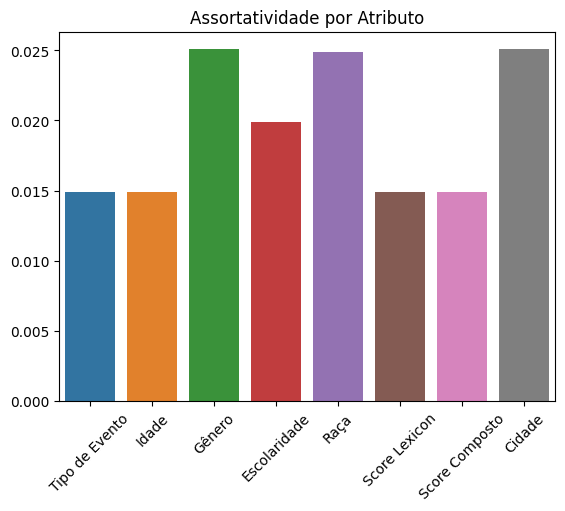
\includegraphics[scale=0.75]{images/assortativity_by_attribute.png}
	\fautor
\end{figure}

Ao analisar os dez usuários com o maior número de postagens na rede, podemos identificar padrões e características que nos ajudam a entender melhor a dinâmica da plataforma e os comportamentos dos usuários mais ativos. Estes usuários, devido à sua alta atividade, têm o potencial de influenciar significativamente a percepção e o sentimento geral da comunidade.

\begin{table}[h]
	\centering
	\caption{Detalhes dos usuários mais ativos}
	\begin{tabular}{|c|c|c|c|c|c|c|c|c|}
		\hline
		ID     & Eigencentrality & Seguidores & Seguindo & Postagens & Score Médio & Gênero & Idade & Raça \\
		\hline
		318649 & 0.0585          & 24         & 5        & 12287.0   & -0.011      & M      & 38    & -    \\
		\hline
		240336 & 0.0532          & 13         & 4        & 11609.0   & 0.03        & M      & 49    & P    \\
		\hline
		425243 & 0.0422          & 15         & 15       & 5310.0    & -0.001      & M      & 48    & P    \\
		\hline
		216238 & 0.1354          & 72         & 17       & 4490.0    & -0.055      & M      & 59    & P    \\
		\hline
		186310 & 0.2552          & 133        & 406      & 4185.0    & -0.052      & M      & 52    & N    \\
		\hline
		76184  & 0.0447          & 74         & 56       & 4031.0    & -0.079      & M      & 31    & N    \\
		\hline
		43341  & 0.0261          & 64         & 24       & 3621.0    & -0.165      & M      & 40    & B    \\
		\hline
		194422 & 0.0234          & 28         & 14       & 2911.0    & -0.329      & O      & 28    & -    \\
		\hline
		253059 & 0.0624          & 26         & 6        & 1698.0    & 0.082       & M      & 48    & B    \\
		\hline
		200628 & 0.0341          & 43         & 0        & 1550.0    & -0.393      & M      & 36    & B    \\
		\hline
	\end{tabular}
\end{table}

Os dois usuários que lideram em número de postagens, com IDs 318649 e 240336, demonstram uma presença significativa na rede, com 12287 e 11609 postagens, respectivamente. No entanto, a influência na rede não se restringe apenas ao volume de postagens. A centralidade de autovetor, que indica a influência de um nó na rede, mostra que o usuário com ID 186310, apesar de estar em quinto lugar em número de postagens, é um dos mais influentes, com uma centralidade de 0.2552. Este usuário destaca-se não só pela sua influência, mas também pelo seu alto número de seguidores, 133, e pelo fato de seguir 406 outros usuários.

O sentimento geral das postagens, representado pelo score médio, varia entre os usuários. Por exemplo, enquanto o usuário com ID 253059 tem um score médio positivo de 0.082, indicando uma tendência a postagens mais positivas, o usuário com ID 194422 tem o score mais negativo de -0.329, sugerindo postagens com um tom mais crítico ou descontente.

Além disso, é interessante observar a diversidade demográfica entre os usuários mais ativos. Temos representantes de diferentes faixas etárias, desde os 28 anos do usuário com ID 194422 até os 59 anos do usuário com ID 216238. Em termos de raça, há uma variedade, com usuários identificados como brancos, negros e pardos. O gênero predominante entre os mais ativos é masculino, com uma exceção identificada como "outros".

A presença de uma ampla gama de scores de sentimento entre os usuários mais ativos é uma indicação saudável de uma comunidade vibrante e multifacetada. Em muitas plataformas online, é comum encontrar usuários que repetidamente postam conteúdo com uma única tonalidade, seja ela positiva, negativa ou neutra. No entanto, a diversidade observada aqui sugere que esses usuários estão engajados em uma variedade de tópicos e situações, refletindo uma gama mais ampla de experiências e sentimentos.

Além disso, essa variedade pode ser vista como um indicativo de autenticidade. Usuários que consistentemente postam com um único tom podem ser percebidos como tendenciosos ou até mesmo como bots. Por outro lado, aqueles cujas postagens refletem uma variedade de sentimentos são mais propensos a serem vistos como genuínos e confiáveis por outros membros da comunidade.

Isso também destaca a importância de não fazer suposições apressadas sobre os usuários com base apenas em sua atividade. Enquanto um alto volume de postagens pode sugerir um usuário muito engajado, a verdadeira natureza de seu engajamento só pode ser compreendida ao se considerar o conteúdo e o sentimento dessas postagens.

A diversidade de sentimentos também pode ser um indicativo de que a plataforma está servindo a seu propósito de fornecer um espaço para discussão e feedback. Se todos os usuários mais ativos tivessem sentimentos uniformemente positivos ou negativos, poderia ser um sinal de que a plataforma está se tornando uma câmara de eco, onde apenas certas opiniões são expressas e reforçadas.

Além disso, essa diversidade pode ser benéfica para os administradores ou moderadores da plataforma. Ao monitorar os sentimentos variados dos usuários mais ativos, eles podem obter insights valiosos sobre áreas de preocupação, bem como aspectos da plataforma ou da comunidade que estão funcionando bem. Isso pode informar decisões sobre modificações na plataforma, campanhas de engajamento ou iniciativas de moderação.

Por fim, é essencial reconhecer que, em qualquer comunidade, a diversidade de opiniões e experiências enriquece o diálogo e a troca de ideias. A presença de usuários ativos com uma variedade de sentimentos sugere uma comunidade dinâmica e engajada, onde os membros se sentem livres para expressar suas opiniões e compartilhar suas experiências, sejam elas positivas, negativas ou neutras.

\section{Resultados e Discussão}

\begin{figure}[!htb]
	\caption{Eigencentrality vs. Número de Posts}
	\label{fig:eigencentrality_vs_number_of_posts}
	\centering
	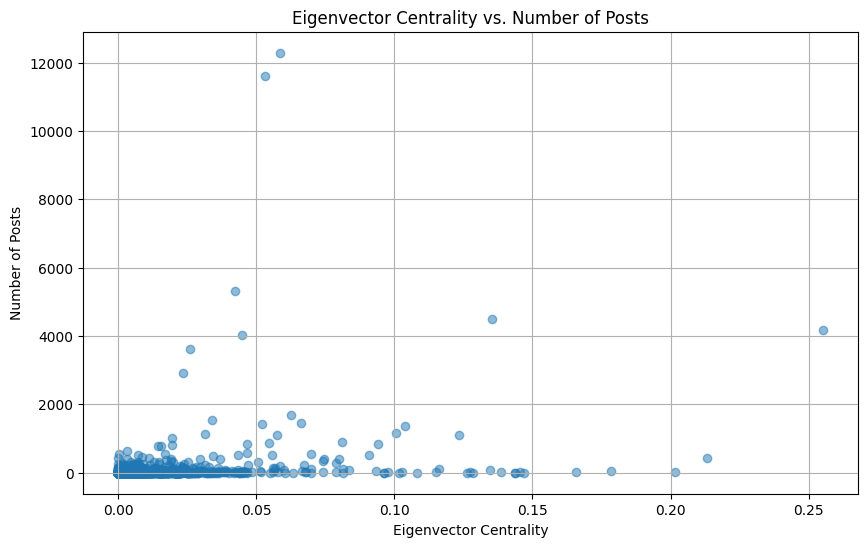
\includegraphics[scale=0.70]{images/eigencentrality_vs_number_of_posts.png}
	\fautor
\end{figure}

Ao longo deste experimento, exploramos a o complexo microcosmo representado pelos sentimentos e opiniões expressas pelos usuários da plataforma Colab. A análise de sentimentos, quando aplicada a plataformas de mídia social, pode revelar insights profundos sobre as percepções, preocupações e satisfações dos usuários. No caso do Colab, essa análise nos permitiu entender melhor a dinâmica da comunidade e as emoções subjacentes às postagens dos usuários.

Primeiramente, a presença de uma distribuição quase equilibrada de sentimentos positivos e negativos desafia a noção comum de que plataformas de feedback tendem a ser dominadas por críticas. Isso sugere que o Colab não é apenas um espaço para reclamações, mas também um fórum onde os usuários reconhecem e apreciam as soluções e melhorias.

A análise dos usuários mais ativos e suas postagens revelou uma diversidade saudável de sentimentos, refutando a ideia de que os usuários mais ativos são unidimensionais em suas postagens. Esta diversidade é um testemunho da autenticidade e do engajamento genuíno dos usuários com a plataforma. Além disso, destaca a importância de considerar o conteúdo e o sentimento das postagens, em vez de se basear apenas no volume de atividade.

A presença de câmaras de eco, onde usuários com sentimentos semelhantes tendem a se agrupar, é uma preocupação em muitas plataformas online. No entanto, a diversidade de sentimentos observada no Colab sugere que a plataforma tem evitado, até certo ponto, essa armadilha. Isso é crucial para garantir que a plataforma continue a ser um espaço para discussão aberta e feedback construtivo.

A análise de redes sociais combinada com a análise de sentimentos também revelou padrões interessantes de conexão e interação entre os usuários. A tendência de usuários com sentimentos semelhantes se conectarem entre si tem implicações significativas para a disseminação de informações e a formação de opiniões dentro da plataforma.

Em conclusão, a análise de sentimentos no Colab ofereceu uma janela única para o coração e a mente da comunidade. Revelou uma comunidade vibrante e engajada, onde os membros se sentem empoderados para expressar suas opiniões e compartilhar suas experiências. À medida que a plataforma continua a crescer e evoluir, será essencial continuar monitorando e compreendendo esses sentimentos para garantir que o Colab permaneça um espaço inclusivo, autêntico e valioso para todos os seus membros.

Até o momento, nossa abordagem para a análise de sentimentos nas postagens do Colab foi baseada em técnicas manuais e ferramentas como o NLTK. Embora tenhamos obtido insights valiosos e estabelecido um score para cada postagem, é evidente que essa metodologia possui limitações em termos de escalabilidade e sustentabilidade, especialmente considerando o volume crescente de dados gerados diariamente na plataforma. Para superar esses desafios e otimizar o processo de análise de sentimentos, é imperativo adotar uma abordagem mais automatizada e robusta. Neste contexto, o aprendizado de máquina emerge como uma solução promissora. Ao utilizar um subconjunto das postagens que já classificamos manualmente - um conjunto de treinamento de aproximadamente 5.000 postagens - podemos treinar um modelo de aprendizado de máquina para realizar a classificação de sentimentos de forma autônoma. Esta abordagem não apenas acelera o processo de análise, mas também garante uma maior consistência e precisão na classificação. No próximo segmento, exploraremos em detalhes a implementação e os benefícios desta metodologia baseada em aprendizado de máquina, delineando como ela pode revolucionar nossa capacidade de entender e interpretar os sentimentos expressos pelos usuários do Colab.

\section{Construção do modelo de classificação supervisionada de sentimentos}

Nessa seção, descrevemos a metodologia empregada para a análise de dados e a construção do modelo de aprendizado de máquina. Apresentamos no \autoref{codigo:sentiment_classifier} uma abordagem para realizar a análise de sentimento em postagens do Colab. Este modelo foi treinado usando um conjunto de dados de treinamento que consiste em postagens de usuário rotuladas como positivas ou negativas. O modelo então aprende a associar certas palavras e frases a sentimentos positivos ou negativos.

Com o intuito de enriquecer o conjunto de dados de treinamento e obter uma visão mais abrangente dos sentimentos expressos nas postagens do Colab, optamos por realizar uma amostragem aleatória do conjunto de dados original, adicionando 2000 eventos ao conjunto de treinamento. Essa abordagem nos permite incorporar uma maior diversidade de exemplos e aumentar a representatividade dos sentimentos presentes nas postagens. Ao selecionar aleatoriamente esses eventos, buscamos evitar qualquer viés de seleção que possa ocorrer ao escolher apenas os piores e melhores scores. Isso nos permite explorar uma variedade mais ampla de nuances de sentimentos que podem estar presentes no conjunto de dados geral.

Além disso, ao combinar esses eventos adicionais com as postagens de scores mais altos e as postagens de scores mais baixos obtidos no experimento anterior na rede das 3 cidades, temos um conjunto de dados de treinamento final composto por 7.000 exemplos. Essa quantidade de dados é considerável e fornece uma base sólida para o treinamento do algoritmo de aprendizado de máquina.

Ao treinar o algoritmo com esse conjunto de dados, esperamos que ele aprenda a associar padrões linguísticos específicos a sentimentos positivos ou negativos, permitindo uma classificação automática mais precisa dos sentimentos expressos nas postagens do Colab. Essa abordagem baseada em aprendizado supervisionado nos permite utilizar os exemplos fornecidos no conjunto de dados de treinamento como referência para o desenvolvimento de um modelo que generalize e capture efetivamente os diferentes matizes de sentimentos presentes nas postagens.

Após a extração de recursos e análise exploratória, dividimos os dados em conjuntos de treinamento e validação. Em seguida, padronizamos os dados para garantir que todas as características tivessem a mesma escala \cite{2000_Jain}. Em seguida, realizamos o treinamento de diferentes modelos de classificação para tentar determinar o modelo mais apropriado para essa aplicação. A seguir, um breve resumo dos modelos utilizados:

\begin{itemize}
	\item \textbf{RandomForestClassifier}: Este algoritmo de aprendizado de máquina supervisionado utiliza o método de "bagging" e a técnica de árvores de decisão. Ele cria várias árvores de decisão e as combina para obter uma predição mais precisa e estável. O RandomForest é útil quando temos um grande conjunto de dados com muitas variáveis de entrada, e é eficaz para evitar o overfitting que pode ocorrer com árvores de decisão individuais \cite[5-32]{2001_Breiman}.
	\item \textbf{LogisticRegression}: A regressão logística é um algoritmo de aprendizado de máquina para classificação. No seu núcleo, é uma regressão, mas com uma função de ativação que transforma a saída em um valor entre 0 e 1. Este modelo é útil quando estamos lidando com problemas de classificação binária e queremos uma probabilidade associada a cada previsão \cite[215-242]{1958_Cox}.
	\item \textbf{DecisionTreeClassifier}: Este algoritmo de aprendizado supervisionado é usado principalmente para problemas de classificação. Ele funciona tanto para variáveis categóricas quanto contínuas. As árvores de decisão são úteis quando queremos um modelo que possa ser facilmente interpretado e explicado \cite[81-106]{1986_Quinlan}.
	\item \textbf{SVC (Support Vector Classifier)}: Este algoritmo de aprendizado de máquina é usado para classificação e regressão, mas é mais comumente usado para tarefas de classificação. O SVC é eficaz em espaços de alta dimensão e é útil quando o número de dimensões é maior do que o número de amostras \cite[273-297]{1995_Cortes}.
	\item \textbf{XGBClassifier (Extreme Gradient Boosting Classifier)}: Este algoritmo de aprendizado de máquina vai além do gradient boosting framework. O XGBoost é útil quando precisamos de um modelo que seja eficiente e tenha um alto desempenho, e é frequentemente usado em competições de ciência de dados devido à sua velocidade e precisão \cite[785-794]{2016_Chen_IP}.
\end{itemize}

Considerando o contexto de análise de sentimentos em busca de câmaras de eco, é crucial escolher um modelo de aprendizado de máquina que seja capaz de capturar com precisão as nuances e polaridades do sentimento expresso nos dados. Diversos estudos têm explorado diferentes modelos para análise de sentimento, cada um com suas próprias vantagens e limitações.

\citeonline{2016_Joshi} utilizaram RandomForest (RF) e Support Vector Machine (SVM) para classificar a polaridade de artigos de notícias financeiras e prever tendências de ações. Eles relataram que ambos os modelos tiveram bom desempenho, com uma precisão de mais de 80\%. Isso sugere que esses modelos podem ser eficazes na análise de sentimentos em câmaras de eco, especialmente quando os dados são ricos em recursos e a tarefa envolve a previsão de tendências com base na polaridade do sentimento.

Por outro lado, \citeonline{2017_Shen_IC} propuseram um modelo combinado de Convolutional Neural Networks (CNNs) e Bidirectional Long Short-Term Memory (BLSTM) para análise de sentimento de críticas de filmes. O modelo alcançou uma precisão de classificação de 89,7\%, que foi significativamente melhor do que a alcançada por CNN ou LSTM sozinhos. Este estudo sugere que modelos de redes neurais profundas, como CNN-BLSTM, podem ser particularmente úteis quando a análise de sentimento envolve a compreensão de sequências de texto complexas, como é frequentemente o caso em câmaras de eco.

\citeonline{2020_Han} propuseram uma função de kernel Fisher baseada em Probabilistic Latent Semantic Analysis para análise de sentimento usando SVM. Os autores relataram uma melhoria na classificação em comparação com os métodos tradicionais. Este estudo sugere que a incorporação de técnicas de análise semântica latente pode melhorar a eficácia dos modelos de análise de sentimento.

Finalmente, \citeonline{2020_Lin} propuseram um modelo de rede neural profunda aprimorado por comparação (Comparison Enhanced Bi-LSTM with Multi-Head Attention) para análise de sentimento. O modelo superou muitos modelos existentes em três conjuntos de dados de análise de sentimento. Este estudo sugere que modelos de atenção, que permitem que o modelo se concentre em partes relevantes do texto, podem ser particularmente eficazes na análise de sentimentos em câmaras de eco.

Em conclusão, embora não haja um único modelo "mais apropriado" para análise de sentimento em câmaras de eco, os estudos acima sugerem que modelos baseados em árvores, como RandomForest, modelos baseados em redes neurais, como CNN-BLSTM, e modelos que incorporam técnicas de análise semântica latente ou atenção podem ser particularmente eficazes.

A acurácia dos modelos foi avaliada utilizando o conjunto de validação e a pontuação F1 foi calculada para medir a precisão do modelo em ambas as classes. Além disso, as matrizes de confusão foram utilizadas para analisar o desempenho de cada modelo na classificação dos sentimentos, permitindo uma compreensão mais detalhada das previsões e erros cometidos.

No que diz respeito à modelagem de aprendizado de máquina, os resultados foram os seguintes:

\begin{itemize}
	\item \textbf{RandomForestClassifier:} O modelo RandomForestClassifier alcançou uma acurácia de treinamento de 0.996 e uma acurácia de validação de 0.172 na última execução em 19 de maio de 2022. Em uma execução anterior em 15 de maio de 2022, a acurácia de treinamento foi de 1.0 e a acurácia de validação foi de 0.14.
	\item \textbf{LogisticRegression:} O modelo LogisticRegression obteve uma acurácia de treinamento de 0.996 e uma acurácia de validação de 0.164 na última execução em 19 de maio de 2022. Em uma execução anterior em 15 de maio de 2022, a acurácia de treinamento foi de 1.0 e a acurácia de validação foi de 0.16.
	\item \textbf{DecisionTreeClassifier:} O modelo DecisionTreeClassifier alcançou uma acurácia de treinamento de 0.996 e uma acurácia de validação de 0.13 na última execução em 19 de maio de 2022. Em uma execução anterior em 15 de maio de 2022, a acurácia de treinamento foi de 1.0 e a acurácia de validação foi de 0.1.
	\item \textbf{SVC:} O modelo SVC obteve uma acurácia de treinamento de 0.395 e uma acurácia de validação de 0.098 na última execução em 19 de maio de 2022. Em uma execução anterior em 15 de maio de 2022, a acurácia de treinamento foi de 0.5906 e a acurácia de validação foi de 0.1.
	\item \textbf{XGBClassifier:} Na última execução em 15 de maio de 2022, o modelo XGBClassifier alcançou uma acurácia de treinamento de 0.3154 e uma acurácia de validação de 0.1.
\end{itemize}

Esses resultados indicam que o modelo RandomForestClassifier teve o melhor desempenho em termos de acurácia de treinamento, enquanto o modelo LogisticRegression teve a melhor acurácia de validação. No entanto, todos os modelos apresentaram uma grande diferença entre as acurácias de treinamento e validação, sugerindo que os modelos podem estar sofrendo de overfitting. Isso significa que os modelos estão se ajustando muito bem aos dados de treinamento, mas não estão generalizando bem para novos dados. Futuras iterações deste trabalho podem explorar técnicas para mitigar o overfitting, como a regularização ou o uso de mais dados de treinamento.

\section{Homofilia e Câmaras de Eco}

A homofilia, termo cunhado por Lazarsfeld e Merton em 1954, refere-se à tendência de indivíduos se associarem a outros que são semelhantes a eles em termos de características, interesses e opiniões. Esse fenômeno é amplamente estudado em diversas áreas, incluindo sociologia, psicologia e ciência das redes, e tem sido observado em várias configurações sociais, desde relacionamentos pessoais até interações online em redes sociais.

A homofilia pode estar intimamente relacionada às câmaras de eco, uma vez que a tendência de buscar semelhanças pode levar à formação de grupos com visões e perspectivas convergentes. Quando os indivíduos se associam principalmente a outros que compartilham suas opiniões, informações e conteúdos que são compartilhados dentro desses grupos tendem a reforçar e amplificar essas visões específicas. Isso cria um ambiente propício para o desenvolvimento de câmaras de eco, onde a diversidade de perspectivas é limitada e as ideias divergentes são escassas. A homofilia pode contribuir para a persistência das câmaras de eco ao restringir a exposição a opiniões contrárias e limitar a troca de informações entre diferentes grupos na rede. Essa dinâmica pode resultar em polarização, falta de entendimento mútuo e até mesmo no fortalecimento de crenças extremas.

Estudos têm destacado a relação entre homofilia e câmaras de eco em diferentes contextos, como a propagação de desinformação em redes sociais ou a formação de bolhas de opinião política. A presença de homofilia nas redes sociais pode contribuir para a criação de "filtros de informação" que reforçam as visões existentes e dificultam a exposição a diferentes perspectivas, aumentando assim a probabilidade de formação de câmaras de eco.

Ao entender o conceito de homofilia e sua relação com as câmaras de eco, podemos explorar métricas e técnicas para identificar e mitigar esses fenômenos nas redes sociais. A análise de métricas de homofilia pode fornecer insights sobre a estrutura das redes sociais e ajudar a compreender como as informações são disseminadas e as opiniões são formadas dentro desses contextos específicos. Essas descobertas podem ser fundamentais para desenvolver estratégias e intervenções que promovam uma maior diversidade de perspectivas, diálogo e compreensão mútua na era digital.

As métricas de homofilia geradas a partir deste experimento podem ajudar a detectar câmaras de eco em um grafo da rede do Colab. Câmaras de eco são fenômenos sociais onde as opiniões e informações são amplificadas ou reforçadas pela comunicação e repetição dentro de um sistema fechado e podem contribuir para a polarização social. Ao identificar e entender estas câmaras de eco, podemos desenvolver estratégias para promover a diversidade de opiniões e a comunicação aberta.

\section{Personas e Scores: Novas Métricas para Análise de Sentimento das Postagens do Colab}

No experimento anterior, conduzimos uma análise detalhada centrada na interação dos usuários na plataforma Colab, utilizando técnicas avançadas de processamento de linguagem natural e análise de redes. A primeira parte dessa análise envolveu a criação de um sistema de score, que atribuiu valores positivos, negativos ou neutros a cada postagem baseado no seu conteúdo textual, levando em consideração não apenas as palavras utilizadas, mas também o uso de emojis e a presença de jargões específicos do contexto do aplicativo.

Esse sistema de score nos permitiu ter uma visão mais aprofundada sobre a natureza das interações na plataforma, identificando padrões de comportamento e sentimentos predominantes nas discussões. Além disso, ao integrar essa análise de sentimentos com a análise de redes, pudemos observar como os sentimentos se propagam através das conexões entre os usuários, criando uma dinâmica complexa e multifacetada de interações.

A partir desse ponto, percebemos que a métrica de score poderia ser levada um passo adiante para desenvolver algo ainda mais significativo. Foi assim que surgiu a ideia de criar "personas", que são representações mais holísticas e generalizadas dos usuários, agrupando-os conforme suas características e comportamentos predominantes na plataforma. Essa nova métrica não apenas leva em consideração os scores individuais das postagens, mas também como esses usuários estão interconectados e como influenciam e são influenciados pela rede como um todo.

As personas, por sua vez, são representações fictícias e generalizadas de grupos de usuários que compartilham características e comportamentos semelhantes. No contexto do Colab, duas personas principais foram identificadas: os 'Helpers' e os 'Complainers'. Os Helpers são caracterizados por um comportamento proativo e colaborativo, envolvendo-se em atividades de ajuda e compartilhamento de informações úteis. Por outro lado, os Complainers têm um comportamento mais crítico ou negativo, expressando insatisfação ou críticas.

Essas personas desempenharam papéis distintos na comunidade do Colab, contribuindo para a colaboração e o aprimoramento contínuo da plataforma. Em um mundo ideal, usuários com essas personas coexistiriam em harmonia, compartilhando informações e opiniões de maneira construtiva. No entanto, em muitos casos, essas personas podem se tornar polarizadas, reforçando suas crenças e limitando a diversidade de perspectivas. Essa polarização pode levar à formação de câmaras de eco, onde os usuários são expostos principalmente a informações e opiniões que confirmam suas crenças existentes, pois interagem primariamente com outros usuários que se encaixam na mesma persona. Ao realizar analises de sentimento e classificar usuários em personas baseadas em suas postagens, ganhamos insights sobre como esses usuários se distribuem na rede, identificando padrões que podem indicar os fatores que influenciam a formação dessas bolhas. Existem de fato bolhas de personas de usuários na rede do Colab? Se existem, será que se trata de um comportamento dos usuários ou as plataformas de mídias sociais, através de um viés algorítimico, têm um papel ativo na formação dessas bolhas? Quais ações o Colab pode tomar para mitigar esses efeitos negativos e promover um discurso mais distribuído e menos polarizado? Essas são algumas das questões que pretendemos responder incorporando métricas provenientes de análise de sentimento no modelo de dados dos usuários.

\subsubsection*{Helpers}

A persona "helper" é caracterizada por um comportamento proativo e colaborativo em uma comunidade online. Esses indivíduos são frequentemente encontrados respondendo a perguntas, oferecendo conselhos e compartilhando informações úteis com outros membros da comunidade. Eles tendem a expressar sentimentos positivos em suas postagens e são motivados pelo desejo de ajudar os outros e contribuir para a comunidade.

Os "helpers" são fundamentais para o sucesso de qualquer comunidade online, pois eles ajudam a criar um ambiente de apoio e colaboração. Eles são frequentemente vistos como líderes informais ou especialistas em suas respectivas áreas de interesse. Eles podem ser motivados por uma variedade de fatores, incluindo o desejo de compartilhar conhecimento, a satisfação de ajudar os outros, ou o reconhecimento e respeito que recebem da comunidade.

\subsubsection*{Complainers}

A persona "complainer" é caracterizada por um comportamento mais crítico ou negativo em uma comunidade online. Esses indivíduos são frequentemente encontrados expressando insatisfação, fazendo reclamações ou criticando outros membros da comunidade ou a comunidade como um todo. Eles tendem a expressar sentimentos negativos em suas postagens e são motivados por uma variedade de fatores, incluindo frustração, descontentamento ou a necessidade de expressar suas opiniões.

Os "complainers" desempenham um papel importante em qualquer comunidade online, pois eles ajudam a identificar problemas, desafios ou áreas de melhoria. Embora suas postagens possam ser percebidas como negativas, elas podem fornecer feedback valioso que pode ser usado para melhorar a comunidade. No entanto, é importante gerenciar e responder adequadamente a esses usuários para evitar a criação de um ambiente negativo ou tóxico.

\subsection*{O papel das personas na Comunidade do Colab}

A presença das personas "Helpers" e "Complainers" dentro do Colab é altamente relevante para o ecossistema dessa plataforma colaborativa. Ambas as personas desempenham papéis distintos e complementares que podem influenciar a experiência do usuário e fornecer insights valiosos para o aprimoramento contínuo do aplicativo. A seguir, são apresentados os argumentos que sustentam a relevância dessas personas específicas:

Os Helpers desempenham um papel fundamental no Colab, pois contribuem ativamente para a comunidade, oferecendo suporte, compartilhando conhecimento e fornecendo soluções para os desafios enfrentados pelos usuários. Eles ajudam a fomentar a colaboração e o aprendizado coletivo, tornando-se recursos valiosos para aqueles que precisam de assistência ou orientação. Sua presença cria um ambiente propício para troca de ideias, resolução de problemas e crescimento mútuo. Ao compartilhar suas habilidades e conhecimentos, os Helpers estabelecem uma cultura de generosidade e reciprocidade dentro da comunidade do Colab. Eles inspiram outros usuários a se envolverem ativamente, encorajando a participação e a colaboração entre os membros. Além disso, a presença de Helpers é essencial para garantir que novos usuários se sintam bem-vindos e apoiados, promovendo assim um ambiente inclusivo e acolhedor.

Embora os Complainers possam ser vistos como usuários críticos ou negativos, sua presença é igualmente importante para o Colab. Essas personas desempenham o papel de destacar problemas, lacunas e áreas de melhoria dentro do aplicativo. Ao expressar suas preocupações e insatisfações, eles fornecem um feedback valioso que pode impulsionar o aprimoramento contínuo da plataforma.

Os Complainers atuam como "sentinelas" da comunidade, chamando a atenção para questões que podem ter sido negligenciadas ou passado despercebidas. Suas críticas construtivas podem levar a melhorias significativas na usabilidade, funcionalidade e qualidade geral do Colab. Além disso, ao abordar e resolver essas preocupações, a equipe responsável pelo desenvolvimento do aplicativo demonstra seu compromisso com a satisfação e o engajamento dos usuários.

A interação entre as personas "Helpers" e "Complainers" no Colab é uma relação simbiótica que impulsiona o crescimento e o aprimoramento contínuo da plataforma. Os Helpers oferecem suporte, orientação e soluções, tornando o ambiente colaborativo e enriquecedor. Por outro lado, os Complainers fornecem feedback crítico e identificam áreas de melhoria, promovendo a evolução e aprimoramento do aplicativo. Essa sinergia entre essas personas complementares é essencial para criar uma comunidade vibrante, responsiva e em constante aprimoramento no Colab.

A partir de uma análise exploratória de sentimento, foram identificadas as personas "Helpers" e "Complainers" dentro do Colab. No entanto, é importante ressaltar que existem outras personas que também podem ser identificadas, como por exemplo, a persona "Explorer", que tem um perfil voltado para a exploração da cidade e reporte dos problemas identificados. Além disso, uma nova persona que poderia ser considerada é a persona "Innovator", alguém que está sempre em busca de novas soluções e ideias inovadoras para melhorar a experiência dos usuários no Colab. A escolha das duas personas mencionadas anteriormente foi baseada nossa capacidade de mensurar e classificar essas personas através da analise de sentimento de suas postagens e também em seu potencial de gerar câmaras de eco, pois representam posições mais antagônicas dentro das comunidades da rede.

Nas próximas páginas, detalharemos as técnicas e metodologias utilizadas para identificar e classificar as personas "Helpers" e "Complainers" dentro do Colab, fornecendo uma visão mais aprofundada sobre a implementação dessas personas e sua contribuição para a análise de dados e aprimoramento da plataforma.

\section{Classificação de usuário por persona}

A construção de um modelo de classificação para análise de sentimentos em plataformas como o Colab é uma tarefa intrincada. A linguagem utilizada pelos usuários é repleta de nuances, jargões específicos, emojis e outros elementos que podem influenciar a interpretação do sentimento. Além disso, a diversidade demográfica dos usuários traz uma riqueza de perspectivas e formas de expressão. O principal desafio é desenvolver um modelo que seja sensível a essas nuances, evitando o overfitting, e que possa generalizar bem para postagens não vistas anteriormente.

Para assegurar uma representação abrangente e equitativa da comunidade do Colab, 5000 postagens foram meticulosamente selecionadas com base em critérios demográficos. Esta seleção garantiu que todas as faixas etárias, gêneros e raças estivessem representados de forma proporcional à distribuição desses grupos entre os usuários do aplicativo. Além disso, levamos em consideração o tamanho das postagens, garantindo uma mistura de postagens longas e curtas. Cada postagem foi então manualmente classificada como 'helper' ou 'complainer', considerando-se o conteúdo, a intenção e as nuances da linguagem.

Do conjunto inicial de postagens, 4000 foram destinadas ao treinamento, mantendo um equilíbrio de 2000 postagens para cada categoria ('helper' e 'complainer'). As 1000 postagens restantes foram reservadas como conjunto de teste. Esta separação assegura que o modelo seja treinado e avaliado em conjuntos distintos, minimizando o risco de overfitting.

A abordagem adotada para a análise de sentimentos e classificação de personas é orientada a objetos, o que facilita a modularização e reutilização do código. O código é estruturado em várias classes, cada uma com responsabilidades específicas. A classe SentimentClassifierModel é responsável pela carga de dados, pré-processamento, vetorização e treinamento de modelos de classificação de sentimentos. A vetorização é realizada usando o CountVectorizer, que converte o texto em uma matriz de contagens de termos/tokens. A classe também suporta vários tipos de modelos, incluindo Floresta Aleatória, Regressão Logística, Árvore de Decisão e KNN, permitindo flexibilidade na escolha do algoritmo.

\begin{figure}
	\centering
	\begin{tikzpicture}[node distance=2cm, auto]
		% Estilos
		\tikzstyle{block} = [rectangle, draw, fill=blue!20, text width=6em, text centered, rounded corners, minimum height=3em]
		\tikzstyle{line} = [draw, -latex']
		% Nós
		\node [block] (init) {Carregar Dados};
		\node [block, below of=init] (preprocess) {Pré-processamento};
		\node [block, below of=preprocess] (vectorize) {Vetorização};
		\node [block, below of=vectorize] (train) {Treinar Modelo};
		\node [block, below of=train] (validate) {Validação Cruzada Estratificada};
		\node [block, below of=validate] (predict) {Predição};
		\node [block, below of=predict] (analysis) {Análise e Visualização};
		% Conexões
		\path [line] (init) -- (preprocess);
		\path [line] (preprocess) -- (vectorize);
		\path [line] (vectorize) -- (train);
		\path [line] (train) -- (validate);
		\path [line] (validate) -- (predict);
		\path [line] (predict) -- (analysis);

	\end{tikzpicture}
	\caption{Workflow de Classificação.}
\end{figure}

A classe ColabSentimentClassifier atua como uma camada de alto nível, integrando a análise de eventos do Colab com o modelo de classificação de sentimentos. Ela carrega os dados dos eventos, inicializa o modelo e atualiza os scores de sentimentos dos usuários. A classe PersonaClassifier é a peça central para a classificação de personas. Ela utiliza o StratifiedKFold para realizar validação cruzada estratificada, garantindo que cada fold tenha uma distribuição semelhante de 'helper' e 'complainer'. Além disso, essa classe oferece métodos para visualização, como a matriz de confusão e a curva ROC.

O código também enfatiza a importância da limpeza e pré-processamento de dados. Funções de preprocessamento são usadas para remover stopwords, realizar stemming e limpar caracteres indesejados. Esta etapa é crucial, pois a qualidade do texto de entrada pode afetar significativamente a performance do modelo. A abordagem modular e orientada a objetos adotada facilita a manutenção, extensão e compreensão do código, permitindo que pesquisadores e desenvolvedores ajustem e expandam facilmente as funcionalidades conforme necessário.

Para avaliar a robustez e a confiabilidade do modelo, foi empregada a técnica de validação cruzada estratificada. A estratificação, neste contexto, refere-se ao processo de dividir o conjunto de treinamento de forma que cada subconjunto (ou "fold") mantenha uma distribuição semelhante de 'helper' e 'complainer'. Esta técnica é essencial para garantir que o modelo seja avaliado de maneira justa e consistente, independentemente da divisão dos dados. Os resultados dessa validação, com acurácias consistentemente altas, fornecem uma indicação da confiabilidade do modelo.

\begin{figure}[htb]
	\centering
	\caption{Resultados da validação do modelo de classificação de personas.}
	\label{fig:persona_results}
	% Primeira imagem em cima
	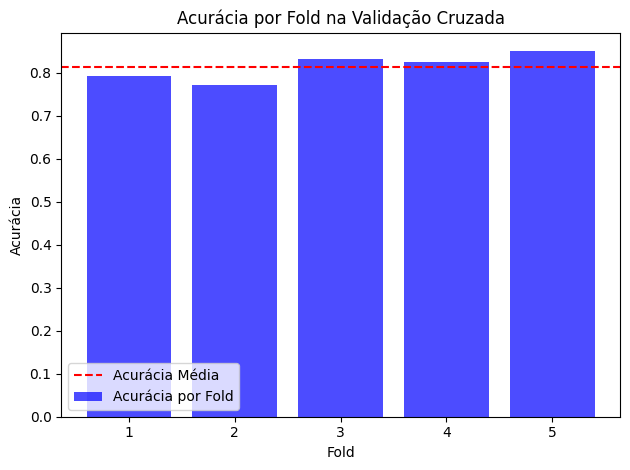
\includegraphics[width=0.8\textwidth]{images/persona_stratified_kfold.png}
	\vspace{1cm} % Espaço vertical entre as imagens
	% Duas imagens embaixo, lado a lado
	\begin{subfigure}[b]{0.49\textwidth}
		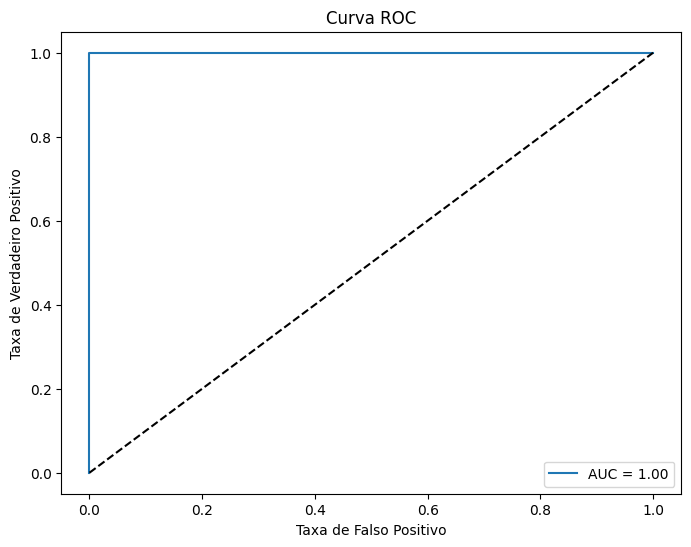
\includegraphics[width=\textwidth]{images/persona_roc.png}
		\caption{Curva ROC}
		\label{fig:persona_roc}
	\end{subfigure}
	~ % Espaço horizontal entre as imagens
	\begin{subfigure}[b]{0.49\textwidth}
		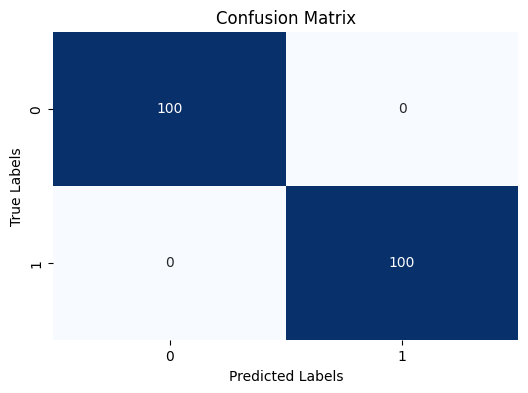
\includegraphics[width=\textwidth]{images/persona_confusion_matrix.png}
		\caption{Matriz de Confusão}
		\label{fig:persona_confusion_matrix}
	\end{subfigure}
	\fautor
\end{figure}

A matriz de confusão e a curva ROC são indicativos claros da eficácia do modelo. Uma matriz de confusão com valores predominantemente nas diagonais e um AUC de 1.0 na curva ROC sugerem um desempenho quase perfeito. No entanto, é crucial reconhecer que, apesar desses resultados promissores, a possibilidade de overfitting não pode ser completamente descartada. A abordagem estratificada e a diversidade do conjunto de treinamento, que inclui postagens de diferentes demografias e tamanhos, servem como contramedidas para esse risco.

O processo de construção do modelo de classificação foi meticuloso e fundamentado em práticas rigorosas. Através da seleção e classificação cuidadosa das postagens, da adoção de técnicas de validação robustas e da análise contínua da confiabilidade, estamos confiantes na capacidade do modelo de classificar postagens de maneira precisa e representativa. Este modelo, aliado à análise de redes e ao sistema de score, oferece uma visão holística e profunda das interações no Colab, abrindo caminho para futuras investigações sobre a dinâmica das comunidades online e o papel das plataformas digitais na formação de opiniões e sentimentos.

\section{Classificação de personas em Modelagem Baseada em Agentes}

A Modelagem Baseada em Agentes (MBA) é uma técnica computacional que tem ganhado interesse em diversas áreas de pesquisa, devido à sua capacidade de simular a interação de agentes autônomos e observar os resultados emergentes dessas interações. A MBA é particularmente útil para estudar sistemas complexos, onde o comportamento global do sistema não pode ser facilmente deduzido a partir do comportamento individual dos agentes.

Agora, consideremos as personas "helpers" e "complainers" em redes sociais. Estas personas, embora não sejam explicitamente mencionadas por Atiqi, podem ser consideradas como agentes dentro da estrutura de MBA. Os "helpers" podem ser vistos como agentes que buscam transmitir mensagens positivas e úteis, enquanto os "complainers" tendem a transmitir mensagens negativas ou críticas. A interação entre essas duas personas pode levar a diferentes dinâmicas de rede e padrões de comunicação. Por exemplo, se os "helpers" são mais influentes ou numerosos, eles podem criar um ambiente mais positivo e cooperativo na rede social. Por outro lado, se os "complainers" são mais influentes ou numerosos, eles podem criar um ambiente mais negativo e crítico.

Além disso, a presença de bots também pode influenciar a dinâmica entre "helpers" e "complainers". Por exemplo, bots programados para agir como "helpers" podem aumentar a positividade e a cooperação na rede, enquanto bots programados para agir como "complainers" podem aumentar a negatividade e a crítica. Portanto, a abordagem de MBA usada por Atiqi se torna uma ferramenta útil para estudar a interação entre "helpers" e "complainers" em redes sociais e entender como essas interações podem influenciar a dinâmica da rede e a formação da opinião pública.